\documentclass[a4paper]{article}

\def\nbook {Fluid Mechanics}
\def\nbookshort {FM}

% Shared preamble. The fallback lets the document build whether the working
% directory is its own folder or the project root.
\IfFileExists{headerfluidmechanics.tex}{\input{headerfluidmechanics}}{\input{../headerfluidmechanics}}

\begin{document}
\maketitle

\newpage
\tableofcontents

\newpage
\section{2 - Cartesian Tensors}

\textbf{Comment on notation}. To denote the \( i \)-th component of a vector, say \( \nabla \times \pmb{v} \), I interchange with the author's notation
\[
	\!\left[ \nabla \times \pmb{v} \right]_{i} \iff \!\left( \nabla \times \pmb{v} \right) \cdot \pmb{e}_{i} 
\]

% QUESTION 1
\qs{2.1}{For three spatial dimensions, rewrite the following expressions in index notation and evaluate or simplify them using the values or parameters given, and the definitions of \( \delta_{ij} \) and \( \epsilon_{ijk} \) wherever possible. In b) through e), \( \pmb{x} \) is the position vector, with components \( x_{i } \).
\begin{enumerate}[label=\textbf{\alph*.}]
	\item \( \pmb{b \cdot c } \) where \( \pmb{b} = \!\left( 1, 4, 17 \right) \) and \( \pmb{c} = \!\left( -4, -3, 1 \right) \).
	\item \( \!\left( \pmb{u} \cdot \nabla \right) \pmb{x} \) where \( \pmb{u} \) a vector with components \( u_{i } \).
	\item \( \nabla \phi  \), where \( \phi = \pmb{h} \cdot \pmb{x} \) and \( \pmb{h} \) is a constant vector with components \( h_{i } \).
	\item \( \nabla \times \pmb{u} \), where \( \pmb{u} = \pmb{\Omega} \times \pmb{x}\) and \( \pmb{\Omega} \) is a constant vector with components \( \pmb{\Omega}_{i} \).
	\item \( \pmb{C} \cdot \pmb{x} \), where
	\[
		\pmb{C} = \begin{Bmatrix}
			1 & 2 & 3\\
			0 & 1 & 2\\
			0 & 0 & 1\\ 
		\end{Bmatrix}
	\]
\end{enumerate}}

\begin{enumerate}[label=\alph*.]
	\item \begin{align*}
		\pmb{b } \cdot \pmb{c } & = b_{1}c_{1} + b_{2}c_{2} + b_{3}c_{3} = \sum_{i} b_{i}c_{i} \equiv b_{i}c_{i} \\
					& = -4 - 12 + 17 \\
					& = 1
	\end{align*}
	\item \begin{align*}
		\!\left( \pmb{u} \cdot \nabla \right)\pmb{x} & = \!\left( u_{1}\frac{\partial }{\partial x_{1}} + u_{2}\frac{\partial }{\partial x_{2}} + u_{3}\frac{\partial }{\partial x_{3}} \right) \!\left( x_{1},x_{2},x_{3} \right) \\
							     & = \!\left( u_{1},u_{2},u_{3} \right) \\
							    \!\left[ \!\left( \pmb{u} \cdot \nabla \right)\pmb{x} \right]_{j} & = u_{i}\frac{\partial x_{j}}{\partial x_{i}} = \delta_{ij}u_{i} = u_{i}
	\end{align*}
	\item Compute \( \pmb{h} \cdot \pmb{x} = h_{1}x_{1} + h_{2}x_{2} + h_{3}x_{3} \).
	\begin{align*}
		\nabla \phi & = \nabla \!\left( \pmb{h} \cdot \pmb{x} \right) \\
		 & = \!\left( \frac{\partial }{\partial x_{1}}\!\left( \pmb{h} \cdot \pmb{x} \right), \frac{\partial }{\partial x_{2}}\!\left( \pmb{h} \cdot \pmb{x} \right), \frac{\partial }{\partial x_{3}}\!\left( \pmb{h} \cdot \pmb{x} \right) \right) = \!\left( h_{1},h_{2},h_{3} \right) \\ 
		\!\left[ \nabla \phi \right]_{j} & = \frac{\partial }{\partial x_{j}}\sum_{i} h_{i}x_{i} = \delta_{ij}h_{i} = h_{i}
	\end{align*}
	\item First compute
	\[
		\!\left[ \pmb{u} \right]_{i} = \!\left[ \pmb{\Omega} \times \pmb{x} \right]_{i} = \sum_{j} \sum_{k} \epsilon_{ijk}\Omega_{j}x_{k} \equiv \epsilon_{ijk}\Omega_{j}x_{k} 
	\]
	Then we can derive
	\begin{align*}
		\!\left[ \nabla \times \pmb{u} \right]_{l} & = \sum_{m} \sum_{n} \epsilon_{lmn}\frac{\partial u_{n}}{\partial x_{m}} \equiv \epsilon_{lmn}\frac{\partial u_{n}}{\partial x_{m}} \\
		 & = \epsilon_{lmn}\frac{\partial }{\partial x_{m}}\!\left( \epsilon_{njk}\Omega_{j}x_{k} \right)
	\end{align*}
	\textbf{Note}: it is nonstandard to have \textbf{more than two} repeating indices. Free indices should only appear \textbf{once}. Remember these as sanity checks!
	\item \begin{align*}
		x'_{i} & = C_{i1}x_{1} + C_{i2}x_{2} + C_{i3}x_{3} = \sum_{j} C_{ij}x_{j} \equiv C_{ij}x_{j} \\
		\pmb{C} \cdot \pmb{x} & = \begin{bmatrix}
			x_{1} + 2x_{2} + 3x_{3} \\
			x_{2} + 2x_{3} \\
			x_{3}
		\end{bmatrix}
	\end{align*}
\end{enumerate}

% QUESTION 6
\qs{2.6}{Convert \( \nabla \times \nabla \rho \) to indicial notation and show that it is zero in Cartesian coordinates for any twice-differentiable scalar function \( \rho \).}

We have from equations (2.22) and (2.24)
\[
	\!\left[ \nabla \times \nabla \rho \right]_{i} = \sum_{j} \sum_{k} \epsilon_{ijk}\frac{\partial }{\partial x_{j}}\!\left( \frac{\partial \rho}{\partial x_{k}} \right) \equiv \epsilon_{ijk}\frac{\partial^2 \rho}{\partial x_{j} \partial x_{k}}
\]
Now, for \( \!\left( i,j,k \right) \) permutations of \( \!\left( 1,2,3 \right) \), fixed \( i \), and dummy indices \( l \), \( m \), we have surviving terms 
\[ 
	\epsilon_{ilm}\!\left( \frac{\partial^{2}\rho}{\partial x_{l}\partial x_{m}} - \epsilon_{iml}\frac{\partial^{2}\rho}{\partial x_{m}\partial x_{l}} \right)
\]
which we have by Clairaut's theorem, \( \partial^{2}\rho / \partial x_{l}\partial x_{m} = \partial^{2}\rho / \partial x_{m}\partial x_{l} \) and \( \epsilon_{ilm} = -\epsilon_{iml} \). Therefore the surviving terms cancel, leaving \( \!\left[ \nabla \times \nabla \rho \right]_{i} = 0 \); by arbitrary choice of \( i \) we establish \( \nabla \times \nabla \rho = \pmb{0} \).

% QUESTION 7
\qs{2.7}{Using indicial notation, show that \( \pmb{a} \times \!\left( \pmb{b} \times \pmb{c} \right) = \!\left( \pmb{a} \cdot \pmb{c} \right)\pmb{b} - \!\left( \pmb{a} \cdot \pmb{b} \right)\pmb{c} \). [\textit{Hint}: Call \( \pmb{d} \equiv \pmb{b} \times \pmb{c} \). Then \( \!\left( \pmb{a} \times \pmb{d} \right)\cdot\pmb{e}_{m} = \epsilon_{pqm}a_{p}\epsilon_{ijq}b_{i}c_{j} \). Using (2.19), show that \( \!\left( \pmb{a} \times \pmb{d} \right) \cdot \pmb{e}_{m} = \!\left( \pmb{a} \cdot \pmb{c} \right)\pmb{b} \cdot \pmb{e}_{m} - \!\left( \pmb{a} \cdot \pmb{b} \right)\pmb{c} \cdot \pmb{e}_{m} \).]}

Define \( \pmb{d} \) as above. Introduce dummy indices \( i \) and \( j \) and free index \( k \). Then the \( k \)-th component of \( \pmb{d} \) is
\[
	d_{k} \equiv \!\left[ \pmb{b} \times \pmb{c} \right]_{k} = \epsilon_{ijk}b_{i}c_{j}
\]
Next, introduce dummy indices \( p \) and \( q \) and free index \( m \). The \( m \)-th component of \( \pmb{a} \times \pmb{d} = \pmb{a} \times \!\left( \pmb{b} \times \pmb{c} \right) \) is
\[
	\!\left[ \pmb{a} \times \pmb{d} \right]_{m} = \epsilon_{pqm}a_{p}\epsilon_{ijq}b_{i}c_{j} 
\]
By (2.19), rewrite the product of the epsilons as 
\[
	\epsilon_{ijq}\epsilon_{pqm} = \epsilon_{ijq}\epsilon_{qmp} = \delta_{im}\delta_{jp} - \delta_{ip}\delta_{jm} 
\]
which leaves us with
\begin{align*}
	\!\left[ \pmb{a} \times \!\left( \pmb{b} \times \pmb{c} \right) \right]_{m} & = \!\left( \delta_{im}\delta_{jp} - \delta_{ip}\delta_{jm} \right)a_{p}b_{i}c_{j} \\
	 & = \!\left( \delta_{jp}a_{p}c_{j} \right)b_{m} - \!\left( \delta_{ip}a_{p}b_{i} \right)c_{m} \\ 
	 & = \!\left[ \!\left( \pmb{a} \cdot \pmb{c} \right)\pmb{b} - \!\left( \pmb{a} \cdot \pmb{b} \right)\pmb{c} \right]_{m}
\end{align*}

% QUESTION 9
\qs{2.9}{Prove the following relationships: \( \delta_{ij}\delta_{ij} = 3 \), \( \epsilon_{pqr}\epsilon_{pqr} = 6 \), and \( \epsilon_{pqi}\epsilon_{pqj} = 2 \delta_{ij} \).}
For fixed indices:
\begin{enumerate}[label=(\alph*)]
	\item Note that either \( \delta_{ij} \) is \( 0 \) or \( 1 \), so we may reduce \( \delta_{ij}\delta_{ij} \) to \( \delta_{ij} \).
	\item Extending this logic a bit, either \( \epsilon_{pqr} \) is \( -1 \), \( 0 \), or \( 1 \). The product \( \epsilon_{pqr}\epsilon_{pqr} \) is either \( 0 \) or \( 1 \), so we may reduce to \( \abs{\epsilon_{pqr}} \).
	\item For fixed \( i \) and \( \epsilon_{pqi} \) non-zero, the pair \( \!\left( p,q \right) \) has \( 2! = 2 \) orderings. Now, suppose \( i \neq j \). Keeping the constraint that \( \epsilon_{pqj} \neq 0 \) also, we find ourselves stuck, as \( j \) cannot equal any of \( p \), \( q \), or \( i \). Thus a non-zero term forces \( i = j \). From our earlier fact that \( \!\left( p,q \right) \) has two permutations, \( \epsilon_{pqi}\epsilon_{pqj} \) has two non-zero index configurations for fixed \( i = j \).
\end{enumerate}
Using these insights, sum over all index values in each identity to derive
\begin{align*}
	\delta_{ij}\delta_{ij} & = \delta_{ij} = \delta_{11} + \delta_{22} + \delta_{33} = 3 \\
	\epsilon_{pqr}\epsilon_{pqr} & = \abs{\epsilon_{pqr}} = \lvert S_3 \rvert = 6 \\ 	       \epsilon_{pqi}\epsilon_{pqj} & = 2 \delta_{ij}
\end{align*}
where \( \lvert S_3 \rvert = 3! \) is the cardinality of \( S_{3} \), the symmetric group of permutations of \( \!\left\{ 1,2,3 \right\} \).

% QUESTION 10
\qs{2.10}{Show that \( \pmb{C} \cdot \pmb{C}^{\textsc{T}} = \pmb{C}^{\textsc{T}} \cdot \pmb{C} = \pmb{\delta} \), where \( \pmb{C} \) is the direction cosine matrix and \( \pmb{\delta} \) is the matrix of the Kronecker delta. Any matrix obeying such a relationship is called an \textit{orthogonal matrix} because it represents transformation of one set of orthogonal axes into another.}

Derive \( \!\left[ \pmb{C} \cdot \pmb{C}^{\textsc{T}} \right]_{ij} \)  as 
\[
	\!\left[ \pmb{C} \cdot \pmb{C}^{\textsc{T}} \right]_{ij} = C_{ik}C_{jk} 
\]
and \( \!\left[ \pmb{C}^{\textsc{T}} \cdot \pmb{C} \right]_{ij} \) as 
\[
	\!\left[ \pmb{C}^{\textsc{T}} \cdot \pmb{C} \right]_{ij} = C_{ki}C_{kj} 
\]
Using the definition that \( C_{ij} = \pmb{e}_{i} \cdot \pmb{e}'_{j} \) for unit vectors in the original and rotated coordinate system, where we clarify that the \( k \)-th component of \( \pmb{e}_{i} \) in the rotated coordinate system is \( \!\left[ \pmb{e}_{i} \right]'_{k} = \pmb{e}_{i} \cdot \pmb{e}'_{k} \).
\begin{align*}
	C_{ik}C_{jk} & = \sum_{k} \!\left( \pmb{e}_{i} \cdot \pmb{e}'_{k} \right)\!\left( \pmb{e}_{j} \cdot \pmb{e}'_{k} \right) \\
		     & = \sum_{k} \!\left[ \pmb{e}_{i} \right]'_{k}\!\left[ \pmb{e}_{j} \right]'_{k} \\
		     & = \pmb{e}_{i} \cdot \pmb{e}_{j} = \delta_{ij} \\
	C_{ki}C_{kj} & = \sum_{k} \!\left( \pmb{e}_{k} \cdot \pmb{e}'_{i} \right)\!\left( \pmb{e}_{k} \cdot \pmb{e}'_{j} \right) \\
		     & = \sum_{k}\!\left[ \pmb{e}'_{i} \right]_{k}\!\left[ \pmb{e}'_{j} \right]_{k} \\
		     & = \pmb{e}'_{i} \cdot \pmb{e}'_{j} = \delta_{ij}
\end{align*}
where we appeal to the invariance of the dot product under coordinate rotation, proving the desired result.

\vspace{12pt}

% QUESTION 11
\qs{2.11}{Show that for a second-order tensor \( \pmb{A} \), the following quantities are invariant under a rotation of axes:
\begin{align*}
	I_{1} & = A_{ii} \\
	I_{2} & = \det \begin{vmatrix}
		A_{11} & A_{12} \\
		A_{21} & A_{22}
	\end{vmatrix} + 
	\det \begin{vmatrix}
		A_{22} & A_{23} \\
		A_{32} & A_{33}
	\end{vmatrix} + 
	\det \begin{vmatrix}
		A_{11} & A_{13} \\
		A_{31} & A_{33}
	\end{vmatrix},
	\text{and} \\
		I_{3} & = \det \!\left( A_{ij} \right)
\end{align*}
[\textit{Hint}: Use the result of Exercise 2.10 and the transformation rule (2.12) to show that \( I'_{1} = A'_{ii} = A_{ii} = I_{1} \). Then show that \( A_{ij}A_{ji} \) and \( A_{ij}A_{jk}A_{ki} \) are also invariants. In fact, \textit{all} contracted scalars of the form \( A_{ij}A_{jk}\cdots A_{mi} \) are invariants. Finally, verify that \( I_{2} = \frac{1}{2}\!\left[ I^{2}_{1} - A_{ij}A_{ji} \right] \), and \( I_{3} = \frac{1}{3}\!\left[ A_{ij}A_{jk}A_{ki} - I_{1}A_{ij}A_{ji} + I_{2}A_{ii} \right] \). Because the right-hand sides are invariant, so are \( I_{2} \) and \( I_{3} \).]}

By the transformation rule (2.12) and exercise 2.10,
\[
	I'_{1} = A'_{ii} = \underbrace{C_{mi}C_{ni}}_{\delta_{mn}}A_{mn} = \delta_{mn}A_{mn}
\]
Now, \( \delta_{mn} = 1 \) only when \( m = n \), so we may set both equal to \( i \) and conclude
\[
	I'_{1} = A'_{ii} = A_{ii} = I_{1}
\]
We call \( I_{1} \) the \textbf{trace}. In general, we can show that \( A_{ij}A_{ji} \) is also invariant. Similarly, write from the transformation rule
\begin{align*}
	A'_{ij}A'_{ji} & = C_{mi}C_{nj}A_{mn}C_{kj}C_{li}A_{kl} \\ 
		       & = \underbrace{C_{mi}C_{li}}_{\delta_{ml}}A_{mn}\underbrace{C_{nj}C_{kj}}_{\delta_{nk}}A_{kl}
\end{align*}
where a non-zero product is guaranteed only when \( m = l \) and \( n = k \). Set \( m = l = i \) and \( n = k = j \) to conclude \( A'_{ij}A'_{ji} = A_{ij}A_{ji} \).

For a finite number of terms, we can prove \( A'_{ij}A'_{jk} \cdots A'_{mi} = A_{ij}A_{jk} \cdots A_{mi} \). Do so by observing
\[
	A'_{ij}A'_{jk} \cdots A'_{mi} = \textcolor{red}{C_{oi}}\textcolor{blue}{C_{nj}}A_{on}\textcolor{blue}{C_{fj}}\textcolor{green}{C_{gk}}A_{fg} \cdots C_{pm}\textcolor{red}{C_{qi}}A_{pq}
\]
By pairing terms of the same color, we can collapse the product into sequences of \( C_{ik}C_{jk} = \delta_{ij} \), which when applied with the aforementioned logic, produce the ``chain'' of \( A \)'s where the second index of one term is the first index of the successive term.

For the final phase, we show that 
\[
	I_{2} = \frac{1}{2}\!\left[ I^{2}_{1} - A_{ij}A_{ji} \right] 
\]
From the definition of \( I_{2} \), compute
\begin{align*}
	I_{2} & = \!\left( A_{11}A_{22} - A_{12}A_{21} \right) + \!\left( A_{22}A_{33} - A_{23}A_{32} \right) + \!\left( A_{11}A_{33} - A_{13}A_{31} \right) \\
	 & = \frac{1}{2}\sum_{i}\sum_{j} \!\left( A_{ii}A_{jj} - A_{ij}A_{ji} \right) \\ 
	 & = \frac{1}{2}\!\left( A_{ii}A_{jj} - A_{ij}A_{ji} \right) \\
	 & = \frac{1}{2}\!\left( I^{2}_{1} - A_{ij}A_{ji} \right)
\end{align*}
where the \( 1/2 \) term arises from double counting in the double sum whenever \( i \neq j \). In the case when \( i = j \), the term vanishes. From the fact that each term on the right-hand side of \( I_{2} \) is invariant under transformation, we conclude \( I'_{2} = I_{2} \).

Lastly, for \( I_{3} \), note that the determinant of a 3-by-3 matrix is given by
\[
	\frac{1}{6}\epsilon_{ijk}\epsilon_{pqr}A_{ip}A_{jq}A_{kr} 
\]
To simplify the product of permutation symbols, we introduce an alternate definition, expressed in terms of the determinant of a matrix of Kronecker deltas:
\[
	\epsilon_{ijk} = \det \begin{vmatrix}
		\pmb{e}_{i} \\
		\pmb{e}_{j} \\
		\pmb{e}_{k} 
	\end{vmatrix} =
	\det \begin{vmatrix}
		\delta_{i1} & \delta_{i2} & \delta_{i3} \\
		\delta_{j1} & \delta_{j2} & \delta_{j3} \\
		\delta_{k1} & \delta_{k2} & \delta_{k3}
	\end{vmatrix}
\]
The product is thus the determinant of the matrix product
\begin{align*}
	\epsilon_{ijk}\epsilon_{pqr} & = \det \begin{vmatrix}
		\pmb{e}_{i} \cdot \pmb{e}_{p} & \pmb{e}_{i} \cdot \pmb{e}_{q} & \pmb{e}_{i} \cdot \pmb{e}_{r} \\
		\pmb{e}_{j} \cdot \pmb{e}_{p} & \pmb{e}_{j} \cdot \pmb{e}_{q} & \pmb{e}_{j} \cdot \pmb{e}_{r} \\
		\pmb{e}_{k} \cdot \pmb{e}_{p} & \pmb{e}_{k} \cdot \pmb{e}_{q} & \pmb{e}_{k} \cdot \pmb{e}_{r}
	\end{vmatrix} \\
				     & =
	\det \begin{vmatrix}
		\delta_{ip} & \delta_{iq} & \delta_{ir} \\
		\delta_{jp} & \delta_{jq} & \delta_{jr} \\
		\delta_{kp} & \delta_{kq} & \delta_{kr}
	\end{vmatrix} \\
				     & = \delta_{ip}\!\left( \delta_{jq}\delta_{kr} - \delta_{jr}\delta_{kq} \right) - \delta_{iq}\!\left( \delta_{jp}\delta_{kr} - \delta_{jr}\delta_{kp}\right) + \delta_{ir}\!\left( \delta_{jp}\delta_{kq} - \delta_{jq}\delta_{kp} \right)
\end{align*}
The next step is some accounting tedium. Essentially, we must figure out all of the ways we can set the triplet \( \!\left( p,q,r \right) \) equal to \( \!\left( i,j,k \right) \). There are six such ways of doing so: in the current order, set equal by holding position, and then ``shifting'' once to the left or once to the right. The other three arise from flipping the order of the first triplet, and once more holding or shifting; these beget the sign change as well from flipping the order of the Levi-Civita indices. 

If you are familiar with the language of dihedral groups, particularly the isomorphism \( S_{3} \cong D_{3} \) (relating the structure of the symmetric group of three elements and rotation and reflection of a triangle), you will notice some similarities here. Our next task is to evaluate the Levi-Civita product term by term and reduce.

\begin{center}
	\renewcommand{\arraystretch}{1.8}
	\setlength{\arraycolsep}{10pt}
	\begin{tabular}{|c||c|}
		\hline
		\rule[-1.2em]{0pt}{3em}
		Term & Simplification \\
		\hline\hline
		\rule[-1.2em]{0pt}{3em}
		\( \frac{1}{6}\delta_{ip}\delta_{jq}\delta_{kr}A_{ip}A_{jq}A_{kr} \) & \( \textcolor{red}{\frac{1}{6}A_{ii}A_{jj}A_{kk}} \) \\
		\hline
		\rule[-1.2em]{0pt}{3em}
		\( -\frac{1}{6}\delta_{ip}\delta_{jr}\delta_{kq}A_{ip}A_{jq}A_{kr} \) & \( \textcolor{blue}{-\frac{1}{6}A_{ii}A_{jk}A_{kj}} \) \\
		\hline
		\rule[-1.2em]{0pt}{3em}
		\( -\frac{1}{6}\delta_{iq}\delta_{jp}\delta_{kr}A_{ip}A_{jq}A_{kr} \) & \( \textcolor{blue}{-\frac{1}{6}A_{ij}A_{ji}A_{kk}} \) \\
		\hline
		\rule[-1.2em]{0pt}{3em}
		\( \frac{1}{6}\delta_{iq}\delta_{jr}\delta_{kp}A_{ip}A_{jq}A_{kr} \) & \( \textcolor{orange}{\frac{1}{6}A_{ik}A_{ji}A_{kj}} \) \\
		\hline
		\rule[-1.2em]{0pt}{3em}
		\( \frac{1}{6}\delta_{ir}\delta_{jp}\delta_{kq}A_{ip}A_{jq}A_{kr} \) & \( \textcolor{orange}{\frac{1}{6}A_{ij}A_{jk}A_{ki}} \) \\
		\hline
		\rule[-1.2em]{0pt}{3em}
				\( -\frac{1}{6}\delta_{ir}\delta_{jq}\delta_{kp}A_{ip}A_{jq}A_{kr} \) & \( \textcolor{blue}{-\frac{1}{6}A_{ik}A_{jj}A_{ki}} \) \\
		\hline
	\end{tabular}
\end{center}

Adding the six terms, which we color-code by virtue of structure of the indices, produces (which we set equal to \( I_{3} \) as at the outset we began with the indicial formula for \( \det \!\left( A_{ij} \right) \))
\[
	I_{3} = \frac{1}{6}\!\left( I^{3}_{1} - 3A_{ii}A_{jk}A_{kj} + 2A_{ij}A_{jk}A_{ki} \right)
\]
The first term of the text's form of \( I_{3} \) is the \( \!\left( 1/3 \right)A_{ij}A_{jk}A_{ki} \) term here. The remaining two terms can be split up to reveal
\begin{align*}
	A_{ii}A_{jj}A_{kk} - 3A_{ii}A_{jk}A_{kj} & = \underbrace{A_{ii}A_{jj}A_{kk} - A_{ii}A_{jk}A_{kj}}_{2A_{ii}\!\left( A_{jj}A_{kk} - A_{jk}A_{kj} \right)} - \underbrace{2A_{ii}A_{jk}A_{kj}}_{2I_{1}A_{ij}A_{ji}} \\
	 & = 2 \!\left( I_{2}A_{ii} - I_{1}A_{ij}A_{ji} \right)
\end{align*}
which takes us to the text's form of \( I_{3} \). At long last, we have proven that every term of \( I_{3} \) is invariant under transformation, and thus \( I'_{3} = I_{3} \).

\newpage

% QUESTION 13
\qs{2.13}{Show that \( \delta_{ij} \) is an isotropic tensor. That is, show that \( \delta'_{ij} = \delta_{ij} \) under rotation of the coordinate system. [\textit{Hint}: Use the transformation rule (2.12) and the results of Exercise 2.10.]}

By the transformation rule (2.12), 
\[
	\delta'_{ij} = C_{mi}C_{nj}\delta_{mn} 
\]
which produces non-zero terms only when \( m = n \). Set both equal to \( k \) and rewrite as 
\[
	\delta'_{ij} = C_{ki}C_{kj}
\]
By the result of 2.10, \( C_{ki}C_{kj} = \delta_{ij} \), establishing the proof that \( \delta_{ij} \) is an isotropic tensor.

\vspace{12pt}

% QUESTION 17
\qs{2.17}{If \( a \) is a positive constant and \( \pmb{b} \) is a constant vector, determine the divergence and the curl of \( \pmb{u} = a \pmb{x} / x^{3} \) and \( \pmb{u} = \pmb{b} \times \!\left( \pmb{x} / x^{2} \right) \) where \( x = \sqrt{x^{2}_{1} + x^{2}_{2} + x^{2}_{3}} \equiv \sqrt{x_{i}x_{i}} \) is the length of \( \pmb{x} \).}

For the divergence, compute
\[
	\nabla \cdot \pmb{u} \equiv \frac{\partial u_{i}}{\partial x_{i}} 
\]
where \( u_{i} = ax_{i}\!\left( x_{j}x_{j} \right)^{-3/2} \) implies
\begin{align*}
	\frac{\partial u_{i}}{\partial x_{i}} & = \frac{\partial }{\partial x_{i}}\!\left[ \frac{ax_{i}}{\!\left( x_{j}x_{j} \right)^{3/2}} \right] \\
					      & = \frac{a \delta_{ii}}{\!\left( x_{j}x_{j} \right)^{3/2}} - \frac{3ax_{i}x_{i}}{\!\left( x_{j}x_{j} \right)^{5/2}} \\
					      & = \frac{3a}{\!\left( x_{j}x_{j} \right)^{3/2}} - \frac{3a}{\!\left( x_{j}x_{j} \right)^{3/2}} \\
					      & = 0 \qquad \!\left( x_{j} \neq 0 \right)
\end{align*}
We refer to this function as the \textbf{inverse-square radial field}, and it shows up ubiquitously in fluid mechanics and electrodynamics. Its curl is
\begin{align*}
	\!\left[ \nabla \times \pmb{u} \right]_{i} & = \epsilon_{ijk}\frac{\partial }{\partial x_{j}}\!\left[ \frac{ax_{k}}{\!\left( x_{l}x_{l} \right)^{3/2}} \right] \\
						   & = \epsilon_{ijk}\!\left[ \frac{a}{\!\left( x_{l}x_{l} \right)^{3/2}}\frac{\partial x_{k}}{\partial x_{j}} - \frac{3ax_{k}}{2\!\left( x_{l}x_{l} \right)^{5/2}} \underbrace{\!\left(\frac{\partial \!\left( x_{l}x_{l} \right)}{\partial x_{j}} \right)}_{2x_{j}} \right] \\ 
	 & = \epsilon_{ijk}\!\left[ \frac{a \delta_{kj}}{\!\left( x_{l}x_{l} \right)^{3/2}} - \frac{3ax_{k}x_{j}}{\!\left( x_{l}x_{l} \right)^{5/2}} \right]
\end{align*}

The first term, which contains \( \epsilon_{ijk}\delta_{kj} \), must vanish, for \( j = k \) has \( \delta_{kj} \neq 0 \) but \( \epsilon_{ijk} = 0 \), and \( j \neq k \) keeps \( \epsilon_{ijk} \neq 0 \) but \( \delta_{kj} = 0 \). The second term, which has \( \epsilon_{ijk}x_{k}x_{j} \), vanishes by contraction of the antisymmetry of \( \epsilon_{ijk} \) and symmetry of \( x_{j}x_{k} \). Therefore \( \!\left[ \nabla \times \pmb{u} \right]_{i} = 0 \).

The second function is
\[
	u_{i} = \epsilon_{ijk}\frac{b_{j}x_{k}}{x_{l}x_{l}} 
\]
which has divergence
\begin{align*}
	\nabla \cdot \pmb{u} & = \frac{\partial }{\partial x_{i}}\!\left( \epsilon_{ijk}\frac{b_{j}x_{k}}{x_{l}x_{l}} \right) \\
	 & = \epsilon_{ijk}\!\left[ \frac{b_{j}}{x_{l}x_{l}}\frac{\partial x_{k}}{\partial x_{i}} - \frac{b_{j}x_{k}}{\!\left( x_{l}x_{l} \right)^{2}}\frac{\partial \!\left( x_{l}x_{l} \right)}{\partial x_{i}} \right] \\ 
	 & = \epsilon_{ijk}\!\left[ \frac{b_{j}\delta_{ki}}{x_{l}x_{l}} - \frac{2b_{j}x_{k}x_{i}}{\!\left( x_{l}x_{l} \right)^{2}} \right]
\end{align*}

In the first term, \( \epsilon_{ijk}\delta_{ki} = 0 \) for any configuration of indices, and by the symmetry-antisymmetry argument, \( \epsilon_{ijk}x_{k}x_{i} \) in the second term implies that the second term vanishes too. Thus \( \nabla \cdot \pmb{u} = 0 \). Lastly, the curl
\begin{align*}
	\!\left[ \nabla \times \pmb{u} \right]_{i} & = \epsilon_{ijk}\frac{\partial }{\partial x_{j}}\!\left( \epsilon_{klm}\frac{b_{l}x_{m}}{x_{n}x_{n}} \right) \\
	 & = \epsilon_{ijk}\epsilon_{klm}\!\left[ \frac{b_{l}}{x_{n}x_{n}}\frac{\partial x_{m}}{\partial x_{j}} - \frac{b_{l}x_{m}}{\!\left( x_{n}x_{n} \right)^{2}}\frac{\partial \!\left( x_{n}x_{n} \right)}{\partial x_{j}} \right] \\ 
	 & = \epsilon_{ijk}\epsilon_{klm}\!\left[ \frac{b_{l}\delta_{mj}}{x_{n}x_{n}} - \frac{2b_{l}x_{m}x_{j}}{\!\left( x_{n}x_{n} \right)^{2}} \right] \\
	 & = \!\left( \delta_{il}\delta_{jm} - \delta_{im}\delta_{jl} \right)\!\left[ \frac{b_{l}\delta_{mj}}{x_{n}x_{n}} - \frac{2b_{l}x_{m}x_{j}}{\!\left( x_{n}x_{n} \right)^{2}} \right] \\
	 & = \frac{b_{l}\delta_{il}\delta_{jm}\delta_{mj}}{x_{n}x_{n}} - \frac{b_{l}\delta_{im}\delta_{mj}\delta_{jl}}{x_{n}x_{n}} - \frac{2b_{l}x_{m}x_{j}\delta_{il}\delta_{jm}}{\!\left( x_{n}x_{n} \right)^{2}} + \frac{2b_{l}x_{m}x_{j}\delta_{im}\delta_{jl}}{\!\left( x_{n}x_{n} \right)^{2}} \\
	 & = \frac{3b_{i}}{x_{n}x_{n}} - \frac{b_{i}}{x_{n}x_{n}} - \frac{2b_{i}}{x_{n}x_{n}} + \frac{2b_{j}x_{i}x_{j}}{\!\left( x_{n}x_{n} \right)^{2}} \\
	 & = \frac{2b_{j}x_{i}x_{j}}{\!\left( x_{n}x_{n} \right)^{2}}
\end{align*}
Thus the curl is 
\[
	\nabla \times \pmb{u} = \frac{2 \!\left( \pmb{b} \cdot \pmb{x} \right)}{x^{4}} \pmb{x}, \qquad \pmb{x} \neq \pmb{0}
\]

% QUESTION 18
\qs{2.18}{Obtain the recipe for the gradient of a scalar function in cylindrical polar coordinates from the integral definition (2.32).}

We will rework (2.32) slightly to take in a scalar function. Let \( \pmb{Q} = \phi\pmb{c} \), where \( \pmb{c} \) is a constant vector and \( \phi \) a scalar function. Using the fact that \( \nabla \cdot \phi \pmb{c} = \pmb{c} \cdot \nabla \phi \), we have
\[
	\pmb{c} \cdot \nabla \phi = \lim\limits_{V \to 0}\pmb{c} \cdot \!\left( \frac{1}{V}\iint_{A} \phi \pmb{n} \, dA \right)
\]
However, since \( c \) may be any arbitrary constant vector, this grants us license to drop the \( \pmb{c} \) from both sides:
\[
	\nabla \phi = \lim\limits_{V \to 0}\frac{1}{V}\iint_{A} \phi \pmb{n} \, dA
\]
For our infinitesimal volume, we consider the wedge bounded by \( \!\left[ r, r + \Delta r \right] \) along \( \pmb{e}_{r} \), \( \!\left[ \theta,\theta + \Delta \theta \right] \) along \( \pmb{e}_{\theta} \), and \( \!\left[ z, z + \Delta z \right] \) along \( \pmb{e}_{z} \). Thus the volume is \( r \Delta r \Delta \theta \Delta z \). The red unit vectors below denote the positive direction for each surface.

\begin{center}
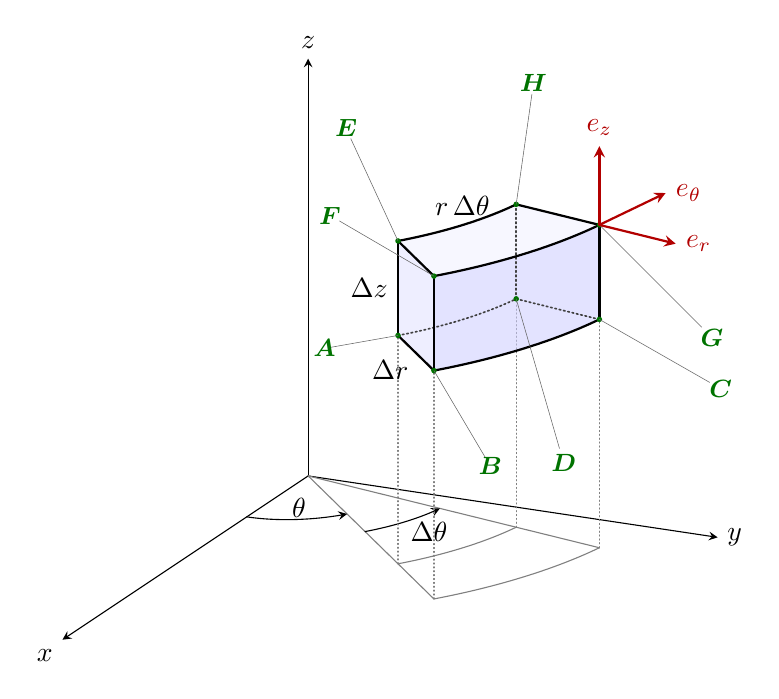
\begin{tikzpicture}[
    x={(-0.6cm,-0.4cm)}, y={(1cm,-0.15cm)}, z={(0cm,1cm)},
    line cap=round, line join=round, >=stealth,
    declare function={
      ra=3; rb=4.2;      % r, r+dr
      ta=50; tb=80;      % theta, theta+dtheta
      za=2.9; zb=4.1;    % z, z+dz
    }]

  % arc at radius #2, from angle #3 to #4, at height #5 (style #1)
  \newcommand{\cylarc}[5][]{%
    \draw[#1] plot[domain=#3:#4, samples=30, variable=\t]
      ({#2*cos(\t)},{#2*sin(\t)},{#5});}

  % axes
  \draw[->] (0,0,0) -- (5.2,0,0) node[below left]  {$x$};
  \draw[->] (0,0,0) -- (0,5.2,0) node[right] {$y$};
  \draw[->] (0,0,0) -- (0,0,5.3) node[above] {$z$};

  % footprint in the z=0 plane
  \draw[gray] (0,0,0) -- ({rb*cos(ta)},{rb*sin(ta)},0);
  \draw[gray] (0,0,0) -- ({rb*cos(tb)},{rb*sin(tb)},0);
  \cylarc[gray]{ra}{ta}{tb}{0}
  \cylarc[gray]{rb}{ta}{tb}{0}
  \cylarc[->]{1.3}{0}{ta}{0}
  \cylarc[->]{1.9}{ta}{tb}{0}
  \node at ({0.95*cos(ta/2)},{0.95*sin(ta/2)},0) {$\theta$};
  \node at ({2.35*cos((ta+tb)/2)},{2.35*sin((ta+tb)/2)},0) {$\Delta\theta$};

  % droplines from footprint to the wedge
  \foreach \r in {ra,rb} \foreach \t in {ta,tb}
    \draw[gray, densely dotted] ({\r*cos(\t)},{\r*sin(\t)},0)
                              -- ({\r*cos(\t)},{\r*sin(\t)},{za});

  % visible faces: theta face (front-left), outer r face, top z face
  \fill[blue!12, opacity=0.55]
    ({ra*cos(ta)},{ra*sin(ta)},{za}) -- ({rb*cos(ta)},{rb*sin(ta)},{za})
    -- ({rb*cos(ta)},{rb*sin(ta)},{zb}) -- ({ra*cos(ta)},{ra*sin(ta)},{zb}) -- cycle;
  \fill[blue!20, opacity=0.55]
    plot[domain=ta:tb, samples=30, variable=\t] ({rb*cos(\t)},{rb*sin(\t)},{za})
    -- plot[domain=tb:ta, samples=30, variable=\t] ({rb*cos(\t)},{rb*sin(\t)},{zb})
    -- cycle;
  \fill[blue!6, opacity=0.55]
    plot[domain=ta:tb, samples=30, variable=\t] ({ra*cos(\t)},{ra*sin(\t)},{zb})
    -- plot[domain=tb:ta, samples=30, variable=\t] ({rb*cos(\t)},{rb*sin(\t)},{zb})
    -- cycle;

  % hidden edges, drawn on top of the faces so the wedge reads as see-through;
  % all three meet at the hidden vertex D
  \begin{scope}[densely dotted, semithick, black!75]
    \cylarc{ra}{ta}{tb}{za}
    \draw ({ra*cos(tb)},{ra*sin(tb)},{za}) -- ({rb*cos(tb)},{rb*sin(tb)},{za});
    \draw ({ra*cos(tb)},{ra*sin(tb)},{za}) -- ({ra*cos(tb)},{ra*sin(tb)},{zb});
  \end{scope}

  % visible edges
  \cylarc[thick]{ra}{ta}{tb}{zb}
  \cylarc[thick]{rb}{ta}{tb}{zb}
  \cylarc[thick]{rb}{ta}{tb}{za}
  \foreach \t in {ta,tb}
    \draw[thick] ({ra*cos(\t)},{ra*sin(\t)},{zb}) -- ({rb*cos(\t)},{rb*sin(\t)},{zb});
  \draw[thick] ({ra*cos(ta)},{ra*sin(ta)},{za}) -- ({rb*cos(ta)},{rb*sin(ta)},{za})
        node[midway, below left=-1pt] {$\Delta r$};
  \draw[thick] ({ra*cos(ta)},{ra*sin(ta)},{za}) -- ({ra*cos(ta)},{ra*sin(ta)},{zb})
        node[midway, left] {$\Delta z$};
  \draw[thick] ({rb*cos(ta)},{rb*sin(ta)},{za}) -- ({rb*cos(ta)},{rb*sin(ta)},{zb});
  \draw[thick] ({rb*cos(tb)},{rb*sin(tb)},{za}) -- ({rb*cos(tb)},{rb*sin(tb)},{zb});
  \node[above] at ({ra*cos((ta+tb)/2)},{ra*sin((ta+tb)/2)},{zb}) {$r\,\Delta\theta$};

  % vertex labels with leader lines: bottom face ABCD (z), top face EFGH (z + dz)
  %   A,E: (r, theta)               B,F: (r+dr, theta)
  %   C,G: (r+dr, theta+dtheta)     D,H: (r, theta+dtheta)
  % \dx,\dy = label offset from the vertex, in cm on the page
  \colorlet{vtx}{green!45!black}   % vertex letter colour
  \begin{scope}[font=\small\bfseries\boldmath, inner sep=1.5pt]
    \foreach \r/\t/\z/\name/\dx/\dy in {
        ra/ta/za/A/-0.85/-0.15,  rb/ta/za/B/0.65/-1.10,
        rb/tb/za/C/1.40/-0.80,   ra/tb/za/D/0.55/-1.90,
        ra/ta/zb/E/-0.60/1.30,   rb/ta/zb/F/-1.20/0.70,
        rb/tb/zb/G/1.30/-1.30,   ra/tb/zb/H/0.20/1.40}
    {
      \fill[vtx] ({\r*cos(\t)},{\r*sin(\t)},{\z}) circle[radius=1pt];
      \draw[very thin, black!60] ({\r*cos(\t)},{\r*sin(\t)},{\z})
            -- ++(\dx cm,\dy cm) node[pos=1.1, text=vtx] {$\name$};
    }
  \end{scope}

  % local unit vectors at the corner (r+dr, theta+dtheta, z+dz)
  \begin{scope}[shift={({rb*cos(tb)},{rb*sin(tb)},{zb})}, red!70!black, thick, ->]
    \draw (0,0,0) -- ({1.1*cos(tb)},{1.1*sin(tb)},0)  node[right] {$\pmb{e}_{r}$};
    \draw (0,0,0) -- ({-1.1*sin(tb)},{1.1*cos(tb)},0) node[right] {$\pmb{e}_{\theta}$};
    \draw (0,0,0) -- (0,0,1.0)                        node[above] {$\pmb{e}_{z}$};
  \end{scope}
\end{tikzpicture}
\end{center}

Following the method in example 2.12, begin with Taylor expanding \( \phi \) from the center of the volume to the center of each side; \textbf{be aware that this will depend on the specified face.} As an example, we derive for faces \( BCFG \) and \( ADEH \):
\begin{align*}
	\!\left[ \phi \right]_{BCFG} & = \phi + \frac{\Delta r}{2}\frac{\partial \phi}{\partial r} + \cdots \\
	\!\left[ \phi \right]_{ADEH} & = \phi - \frac{\Delta r}{2}\frac{\partial \phi}{\partial r} + \cdots
\end{align*}
where the positive and minus signs arise from either a positive or negative displacement from the center of the volume, i.e. in the direction of \( \pmb{n} = \pmb{e}_{r} \) or \( \pmb{n} = -\pmb{e}_{r} \). Put differently, our use of the midpoint rule on each face enables this clean orientation of the anti-parallel normals along the \( r \)-axis. The infinitesimal area on these faces is \( \!\left( r - \Delta r / 2 \right) \Delta \theta \Delta z \) on \( ADEH \) and \( \!\left( r + \Delta r / 2 \right)\Delta \theta \Delta z \) on \( BCFG \). Then \( \phi \pmb{n} \, dA \) is
\begin{align*}
	\!\left( \!\left[ \phi \pmb{n} \right]_{BCFG} + \!\left[ \phi \pmb{n} \right]_{ADEH} \right)dA & = \biggl( \pmb{e}_{r}\!\left[ \phi + \frac{\Delta r}{2}\frac{\partial \phi}{\partial r} + \cdots \right]\!\left( r + \frac{\Delta r}{2} \right) \\
												       & \qquad - \pmb{e}_{r} \!\left[ \phi - \frac{\Delta r}{2}\frac{\partial \phi}{\partial r} + \cdots \right]\!\left( r - \frac{\Delta r}{2} \right) \biggr) \Delta \theta \Delta z \\
												       & = \pmb{e}_{r}\!\left( \phi \Delta r + r \Delta r \frac{\partial \phi}{\partial r} + \cdots \right) \Delta \theta \Delta z \\
												       & = \pmb{e}_{r}\!\left( \frac{\phi}{r} + \frac{\partial \phi}{\partial r} + \cdots \right)r \Delta r \Delta \theta \Delta z
\end{align*}
Analogously, we can compute
\begin{align*}
	\!\left( \!\left[ \phi \pmb{n} \right]_{CDGH} + \!\left[ \phi \pmb{n} \right]_{ABEF} \right)dA & = \biggl( \!\left[ \pmb{e}_{\theta} - \frac{\Delta \theta}{2}\pmb{e}_{r} \right]\!\left[ \phi + \frac{\Delta \theta}{2}\frac{\partial \phi}{\partial \theta} + \cdots \right] \\
												       & \qquad - \!\left[ \pmb{e}_{\theta} + \frac{\Delta \theta}{2}\pmb{e}_{r} \right]\!\left[ \phi - \frac{\Delta \theta}{2}\frac{\partial \phi}{\partial \theta} + \cdots \right] \biggr)\Delta r \Delta z \\
												       & = \!\left[ -\pmb{e}_{r} \phi \Delta \theta + \pmb{e}_{\theta}\!\left( \Delta \theta \frac{\partial \phi}{\partial \theta} + \cdots \right) \right] \Delta r \Delta z \\ 
												       & = \!\left( -\pmb{e}_{r}\frac{\phi}{r} + \pmb{e}_{\theta}\frac{1}{r}\frac{\partial \phi}{\partial \theta} \right) r \Delta r \Delta \theta \Delta z \\
	\!\left( \!\left[ \phi \pmb{n} \right]_{EFGH} + \!\left[ \phi \pmb{n} \right]_{ABCD} \right)dA & = \!\left( \pmb{e}_{z}\!\left[ \phi + \frac{\Delta z}{2}\frac{\partial \phi}{\partial z} + \cdots \right] - \pmb{e}_{z}\!\left[ \phi - \frac{\Delta z}{2}\frac{\partial \phi}{\partial z} + \cdots \right] \right) r \Delta r \Delta \theta \\
												       & = \pmb{e}_{z}\!\left( \frac{\partial \phi}{\partial z} + \cdots \right)r \Delta r \Delta \theta \Delta z
\end{align*}

where the \( \pmb{e}_{\theta} \) directions warrant some discussion. Observe in the diagram below that the normals of the ``opposite'' faces along that axis are not necessarily anti-parallel with one another. As it turns out, the normals are pointing away from \( \pmb{e}_{\theta} \) by some amount; namely, this amount is \( \Delta \theta / 2 \) in the direction of \( -\pmb{e}_{r} \). From the Taylor series expansion of \( \pmb{e}_{\theta} \), this looks like
\[
	\pmb{e}_{\theta}\!\left( \theta \pm \tfrac{\Delta \theta}{2} \right) = \pmb{e}_{\theta} \pm \frac{\Delta \theta}{2}\frac{\partial \pmb{e}_{\theta}}{\partial \theta} + \cdots = \pmb{e}_{\theta} \mp \frac{\Delta \theta}{2}\pmb{e}_{r} + \cdots 
\]
where we use the classic result that \( \partial \pmb{e}_{\theta} / \partial \theta = -\pmb{e}_{r} \).

\begin{center}
\begin{tikzpicture}[
    >=stealth, line cap=round, line join=round,
    declare function={
      ra=3.2; rb=5.2; rm=4.2;   % inner, outer, center radius
      ta=25;  tb=65;  tm=45;    % theta - dtheta/2, theta + dtheta/2, center angle
      hd=20;                    % half-angle dtheta/2 (exaggerated for visibility)
      L=1.6;                    % drawn length of the unit normals
    }]
  \colorlet{vtx}{green!45!black}
  \colorlet{nrm}{red!70!black}
  \colorlet{lean}{blue!70!black}

  % axes and the rays theta = const through the two theta-faces
  \draw[->] (0,0) -- (6.6,0) node[right] {$x$};
  \draw[->] (0,0) -- (0,6.0) node[above] {$y$};
  \draw[gray, dashed] (0,0) -- ({ta}:{rb+1.3});
  \draw[gray, dashed] (0,0) -- ({tb}:{rb+1.3});
  \draw[gray, densely dotted] (0,0) -- ({tm}:{rm});

  % angle marker
  \draw[<->] ({ta}:1.5) arc[start angle=ta, end angle=tb, radius=1.5];
  \node at ({tm}:1.9) {$\Delta\theta$};

  % the box seen from above (top face EFGH)
  \filldraw[thick, fill=blue!12]
    ({ta}:{ra}) arc[start angle=ta, end angle=tb, radius=ra]
    -- ({tb}:{rb}) arc[start angle=tb, end angle=ta, radius=rb] -- cycle;

  % arc lengths: outer face is longer than inner face
  \node[rotate=tm-90, font=\small] at ({tm}:{rb+0.35})
        {$\bigl(r+\tfrac{\Delta r}{2}\bigr)\Delta\theta$};
  \node[rotate=tm-90, font=\small] at ({tm}:{ra-0.35})
        {$\bigl(r-\tfrac{\Delta r}{2}\bigr)\Delta\theta$};

  % vertices (top view: E over A, F over B, G over C, H over D)
  \begin{scope}[font=\small\bfseries\boldmath, text=vtx]
    \fill[vtx] ({ta}:{ra}) circle[radius=1.2pt] node[below]       {$E$};
    \fill[vtx] ({ta}:{rb}) circle[radius=1.2pt] node[below right] {$F$};
    \fill[vtx] ({tb}:{rb}) circle[radius=1.2pt] node[above right] {$G$};
    \fill[vtx] ({tb}:{ra}) circle[radius=1.2pt] node[left]        {$H$};
  \end{scope}

  % basis vectors at the center of the box
  \fill ({tm}:{rm}) circle[radius=1.2pt];
  \draw[->, thick] ({tm}:{rm}) -- ++({tm}:0.6)    node[below right=-3pt, font=\small] {$\pmb{e}_r$};
  \draw[->, thick] ({tm}:{rm}) -- ++({tm+90}:0.6) node[below left=-3pt, font=\small]  {$\pmb{e}_\theta$};

  % --- normal on the face theta + dtheta/2 (CDGH, seen edge-on as HG) ---
  \coordinate (P) at ({tb}:{rm});
  \draw[->, gray, dashed] (P) -- ++({tm+90}:{L*cos(hd)}) coordinate (P1)
        node[midway, above right=-2pt, font=\small, text=gray] {$\pmb{e}_\theta$};
  \draw[->, lean, thick]  (P1) -- ++({tm+180}:{L*sin(hd)})
        node[pos=0.3, above=1pt, font=\small] {$-\tfrac{\Delta\theta}{2}\pmb{e}_r$};
  \draw[->, nrm, very thick] (P) -- ++({tb+90}:{L})
        node[left, font=\small] {$\pmb{n}_{CDGH}$};

  % --- normal on the face theta - dtheta/2 (ABEF, seen edge-on as EF) ---
  \coordinate (Q) at ({ta}:{rm});
  \draw[->, gray, dashed] (Q) -- ++({tm-90}:{L*cos(hd)}) coordinate (Q1)
        node[midway, above right=-2pt, font=\small, text=gray] {$-\pmb{e}_\theta$};
  \draw[->, lean, thick]  (Q1) -- ++({tm+180}:{L*sin(hd)})
        node[midway, right=1pt, font=\small] {$-\tfrac{\Delta\theta}{2}\pmb{e}_r$};
  \draw[->, nrm, very thick] (Q) -- ++({ta-90}:{L})
        node[below left=-2pt, font=\small] {$\pmb{n}_{ABEF}$};

  % --- inset: the two normals added tip to tail ---
  \begin{scope}[shift={(10.6,2.4)}]
    \node[font=\small, align=center] at (-1.1,2.0) {sum of the two\\ $\theta$-face normals};
    \coordinate (S) at (0,0);
    \draw[->, nrm, very thick] (S) -- ++({tb+90}:{1.6*L}) coordinate (S1)
          node[midway, above right=-1pt, font=\small] {$\pmb{n}_{CDGH}$};
    \draw[->, nrm, very thick] (S1) -- ++({ta-90}:{1.6*L}) coordinate (S2)
          node[midway, left=2pt, font=\small] {$\pmb{n}_{ABEF}$};
    \draw[->, lean, very thick] (S) -- (S2);
    \node[lean, font=\small, anchor=north] at (-1.1,-1.45)
          {$\pmb{n}_{CDGH}+\pmb{n}_{ABEF}\approx-\Delta\theta\,\pmb{e}_r$};
  \end{scope}
\end{tikzpicture}
\end{center}

Adding our three results together, dividing by the volume and taking the limit, conclude
\begin{align*}
	\nabla \phi & = \lim\limits_{V \to 0}\frac{1}{V}\iint_{A} \phi \pmb{n} \, dA \\
		    & = \lim\limits_{\substack{\Delta r \to 0 \\ \Delta \theta \to 0 \\ \Delta z \to 0}}\frac{1}{r \Delta r \Delta \theta \Delta z}\!\left[ \pmb{e}_{r}\!\left( \frac{\phi}{r} + \frac{\partial \phi}{\partial r} \right) - \pmb{e}_{r}\frac{\phi}{r} + \pmb{e}_{\theta}\frac{1}{r}\frac{\partial \phi}{\partial \theta} + \pmb{e}_{z}\frac{\partial \phi}{\partial z} + \cdots \right] r \Delta r \Delta \theta \Delta z \\
		    & = \pmb{e}_{r}\frac{\partial \phi}{\partial r} + \pmb{e}_{\theta}\frac{1}{r}\frac{\partial \phi}{\partial \theta} + \pmb{e}_{z}\frac{\partial \phi}{\partial z} 
\end{align*}
where we keep only first-order terms in the last equality. Observe there that when \( \phi \) is constant, \( \nabla \phi = \pmb{0} \), comporting with the result \( \oiint \pmb{n} \, dA = \pmb{0} \).

\vspace{12pt}

% QUESTION 19
\qs{2.19}{Obtain the recipe for the divergence of a vector function in cylindrical polar coordinates from the integral definition (2.32).}

The integral definition of divergence is 
\[
	\nabla \cdot \pmb{Q} = \lim\limits_{V \to 0}\iint_{A} \pmb{n} \cdot \pmb{Q} \, dA 
\]
Building off of our work in 2.18, derive
\begin{align*}
	\!\left( \!\left[ \pmb{n} \cdot \pmb{Q} \right]_{BCFG} + \!\left[ \pmb{n} \cdot \pmb{Q} \right]_{ADEH} \right)dA & = \biggl( \pmb{e}_{r} \cdot \!\left[ \pmb{Q} + \frac{\Delta r}{2}\frac{\partial \pmb{Q}}{\partial r} + \cdots \right]\!\left( r + \frac{\Delta r}{2} \right) \\
												       & \qquad - \pmb{e}_{r} \cdot \!\left[ \pmb{Q} - \frac{\Delta r}{2}\frac{\partial \pmb{Q}}{\partial r} + \cdots \right]\!\left( r - \frac{\Delta r}{2} \right) \biggr) \Delta \theta \Delta z \\
												       & = \pmb{e}_{r} \cdot \!\left( \pmb{Q} \Delta r + r \Delta r \frac{\partial \pmb{Q}}{\partial r} + \cdots \right) \Delta \theta \Delta z \\
												       & = \pmb{e}_{r} \cdot \!\left( \frac{\pmb{Q}}{r} + \frac{\partial \pmb{Q}}{\partial r} + \cdots \right)r \Delta r \Delta \theta \Delta z \\
												       & = \!\left( \frac{Q_{r}}{r} + \frac{\partial Q_{r}}{\partial r} + \cdots \right)r \Delta r \Delta \theta \Delta z \\
	\!\left( \!\left[ \pmb{n} \cdot \pmb{Q} \right]_{CDGH} + \!\left[ \pmb{n} \cdot \pmb{Q} \right]_{ABEF} \right)dA & = \biggl( \!\left[ \pmb{e}_{\theta} - \frac{\Delta \theta}{2}\pmb{e}_{r} \right] \cdot \!\left[ \pmb{Q} + \frac{\Delta \theta}{2}\frac{\partial \pmb{Q}}{\partial \theta} + \cdots \right] \\
												       & \qquad - \!\left[ \pmb{e}_{\theta} + \frac{\Delta \theta}{2}\pmb{e}_{r} \right] \cdot \!\left[ \pmb{Q} - \frac{\Delta \theta}{2}\frac{\partial \pmb{Q}}{\partial \theta} + \cdots \right] \biggr)\Delta r \Delta z \\
												       & = \!\left[ -\pmb{e}_{r} \cdot \pmb{Q} \Delta \theta + \pmb{e}_{\theta} \cdot \!\left( \Delta \theta \frac{\partial \pmb{Q}}{\partial \theta} + \cdots \right) \right] \Delta r \Delta z \\ 
												       & = \!\left( -\frac{Q_{r}}{r} + \frac{Q_{r}}{r} + \frac{1}{r}\frac{\partial Q_{\theta}}{\partial \theta} + \cdots \right) r \Delta r \Delta \theta \Delta z \\
												       & = \!\left( \frac{1}{r}\frac{\partial Q_{\theta}}{\partial \theta} + \cdots \right) r \Delta r \Delta \theta \Delta z \\
	\!\left( \!\left[ \pmb{n} \cdot \pmb{Q} \right]_{EFGH} + \!\left[ \pmb{n} \cdot \pmb{Q} \right]_{ABCD} \right)dA & = \!\left( \pmb{e}_{z} \cdot \!\left[ \pmb{Q} + \frac{\Delta z}{2}\frac{\partial \pmb{Q}}{\partial z} + \cdots \right] - \pmb{e}_{z} \cdot \!\left[ \pmb{Q} - \frac{\Delta z}{2}\frac{\partial \pmb{Q}}{\partial z} + \cdots \right] \right) r \Delta r \Delta \theta \\
												       & = \!\left( \frac{\partial Q_{z}}{\partial z} + \cdots \right)r \Delta r \Delta \theta \Delta z
\end{align*}
where a note is needed in the derivation of the integrand along the \( \pmb{e}_{\theta} \) faces. In particular, it is generally incorrect that
\[
	\pmb{e}_{\theta} \cdot \frac{\partial \pmb{Q}}{\partial \theta} = \frac{\partial Q_{\theta}}{\partial \theta}
\]
However, referring to the component definition of \( \pmb{Q} \)
\[
	\pmb{Q} = Q_{r}\pmb{e}_{r} + Q_{\theta}\pmb{e}_{\theta} + Q_{z}\pmb{e}_{z} 
\]
and differentiating 
\[
	\frac{\partial \pmb{Q}}{\partial \theta} = Q_{r}\frac{\partial \pmb{e}_{r}}{\partial \theta} + \pmb{e}_{\theta}\frac{\partial Q_{\theta}}{\partial \theta} + Q_{\theta}\frac{\partial \pmb{e}_{\theta}}{\partial \theta} = \!\left( Q_{r} + \frac{\partial Q_{\theta}}{\partial \theta} \right)\pmb{e}_{\theta} + \!\left( \frac{\partial Q_{r}}{\partial \theta} - Q_{\theta} \right)\pmb{e}_{r} + \frac{\partial Q_{z}}{\partial \theta}\pmb{e}_{z}
\]
We can clearly see that
\[
	\pmb{e}_{\theta} \cdot \frac{\partial \pmb{Q}}{\partial \theta} = Q_{r} + \frac{\partial Q_{\theta}}{\partial \theta} 
\]
This arises from the fact that \( \partial \pmb{e}_{r} / \partial \theta = \pmb{e}_{\theta} \) (namely, that \( \pmb{e}_{r} \) is defined in terms of \( \theta \)).

With that out of the way, sum each piece as 
\begin{align*}
	\nabla \cdot \pmb{Q} & = \lim\limits_{V \to 0}\frac{1}{V}\iint_{A} \pmb{n} \cdot \pmb{Q} \, dA \\
			     & = \lim\limits_{\substack{\Delta r \to 0 \\ \Delta \theta \to 0 \\ \Delta z \to 0}} \frac{1}{r \Delta r \Delta \theta \Delta z}\!\left[ \frac{Q_{r}}{r} + \frac{\partial Q_{r}}{\partial r} + \frac{1}{r}\frac{\partial Q_{\theta}}{\partial \theta} + \frac{\partial Q_{z}}{\partial z} + \cdots \right] r \Delta r \Delta \theta \Delta z \\ 
			     & = \frac{1}{r}\!\left[ \frac{\partial \!\left( rQ_{r} \right)}{\partial r} + \frac{\partial Q_{\theta}}{\partial \theta} \right] + \frac{\partial Q_{z}}{\partial z}
\end{align*}
Notably, the derivation of the divergence using the integral definition exposes the unequal faces along the \( r \)-axis as the source of the \( Q_{r} / r \) that emerges in the divergence.

\vspace{12pt}

% QUESTION 20
\qs{2.20}{Obtain the recipe for the divergence of a vector function in spherical polar coordinates from the integral definition (2.32).}

We illustrate our infinitesimal wedge in spherical coordinates below. The first key conceptual difference to understand is as follows: where the infinitesimal wedge in cylindrical coordinates did not have anti-parallel norms on opposite faces along the \( \theta \) axis, in spherical coordinates this manifests in two places, the \( \theta \) and \( \phi \) axes. The infinitesimal volume is thus \( r^{2}\sin\!\left(\theta\right)\Delta r \Delta \theta \Delta \phi \).

\begin{figure}[h]
  \centering
  % ---------- left: edge lengths and angles ----------
  \begin{minipage}[t]{0.49\textwidth}
    \centering
    \resizebox{\linewidth}{!}{%
      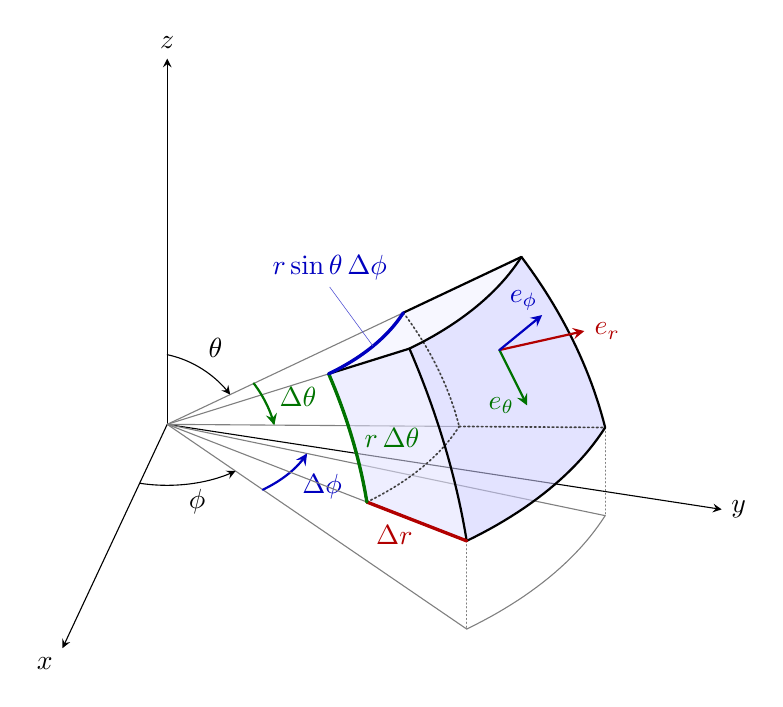
\begin{tikzpicture}[
          % orthographic view (azimuth 15 deg, elevation 35 deg), scaled by 1.35
          x={(-0.35cm,-0.748cm)}, y={(1.304cm,-0.2cm)}, z={(0cm,1.106cm)},
          line cap=round, line join=round, >=stealth,
          declare function={
            ra=3.0;  rb=4.5;     % r,     r + dr
            tha=52;  thb=77;     % theta, theta + dtheta   (polar angle, from +z)
            pa=55;   pb=85;      % phi,   phi + dphi       (azimuth, from +x)
            rm=4.5;  thm=58; pm=70;   % where the unit vectors are drawn (on the outer face)
          }]
        \def\D{\Delta}   % change to d for differentials
        % one colour per coordinate direction
        \colorlet{cr}{red!70!black}
        \colorlet{cth}{green!45!black}
        \colorlet{cph}{blue!75!black}

        % point at (r, theta, phi)
        \newcommand{\sph}[3]{({#1*sin(#2)*cos(#3)},{#1*sin(#2)*sin(#3)},{#1*cos(#2)})}
        % arc in theta at fixed r=#2, phi=#3, from theta=#4 to #5
        \newcommand{\tharc}[5][]{\draw[#1] plot[domain=#4:#5, samples=25, variable=\t]
            ({#2*sin(\t)*cos(#3)},{#2*sin(\t)*sin(#3)},{#2*cos(\t)});}
        % arc in phi at fixed r=#2, theta=#3, from phi=#4 to #5
        \newcommand{\pharc}[5][]{\draw[#1] plot[domain=#4:#5, samples=25, variable=\t]
            ({#2*sin(#3)*cos(\t)},{#2*sin(#3)*sin(\t)},{#2*cos(#3)});}

        % axes
        \draw[->] (0,0,0) -- (3.8,0,0) node[below left] {$x$};
        \draw[->] (0,0,0) -- (0,5.4,0) node[right] {$y$};
        \draw[->] (0,0,0) -- (0,0,4.2) node[above] {$z$};

        % azimuth construction in the z=0 plane
        \draw[gray] (0,0,0) -- ({rb*sin(thb)*cos(pa)},{rb*sin(thb)*sin(pa)},0);
        \draw[gray] (0,0,0) -- ({rb*sin(thb)*cos(pb)},{rb*sin(thb)*sin(pb)},0);
        \draw[gray] plot[domain=pa:pb, samples=25, variable=\t]
            ({rb*sin(thb)*cos(\t)},{rb*sin(thb)*sin(\t)},0);
        \draw[->] plot[domain=0:pa, samples=25, variable=\t] ({1.0*cos(\t)},{1.0*sin(\t)},0);
        \draw[->, cph, thick] plot[domain=pa:pb, samples=25, variable=\t] ({1.4*cos(\t)},{1.4*sin(\t)},0);
        \node at ({1.3*cos(pa/2)},{1.3*sin(pa/2)},0) {$\phi$};
        \node[text=cph] at ({1.78*cos((pa+pb)/2)},{1.78*sin((pa+pb)/2)},0) {$\D\phi$};

        % droplines from the two lower outer corners to the z=0 plane
        \foreach \p in {pa,pb}
          \draw[gray, densely dotted] \sph{rb}{thb}{\p}
              -- ({rb*sin(thb)*cos(\p)},{rb*sin(thb)*sin(\p)},0);

        % rays from the origin to the four inner corners (shows the taper)
        \foreach \t/\p in {tha/pa, tha/pb, thb/pa, thb/pb}
          \draw[gray, thin] (0,0,0) -- \sph{ra}{\t}{\p};

        % polar angle markers, in the half-plane phi = pb
        \tharc[->]{0.8}{pb}{0}{tha}
        \tharc[->, cth, thick]{1.1}{pb}{tha}{thb}
        \path \sph{1.1}{tha/2}{pb} node {$\theta$};
        \path \sph{1.45}{(tha+thb)/2}{pb} node[text=cth] {$\D\theta$};

        % visible faces: phi face (front), theta face (top), outer r face
        \fill[blue!12, opacity=0.55]
          plot[domain=tha:thb, samples=25, variable=\t] ({ra*sin(\t)*cos(pa)},{ra*sin(\t)*sin(pa)},{ra*cos(\t)})
          -- plot[domain=thb:tha, samples=25, variable=\t] ({rb*sin(\t)*cos(pa)},{rb*sin(\t)*sin(pa)},{rb*cos(\t)})
          -- cycle;
        \fill[blue!6, opacity=0.55]
          plot[domain=pa:pb, samples=25, variable=\t] ({ra*sin(tha)*cos(\t)},{ra*sin(tha)*sin(\t)},{ra*cos(tha)})
          -- plot[domain=pb:pa, samples=25, variable=\t] ({rb*sin(tha)*cos(\t)},{rb*sin(tha)*sin(\t)},{rb*cos(tha)})
          -- cycle;
        \fill[blue!20, opacity=0.55]
          plot[domain=pa:pb, samples=25, variable=\t] ({rb*sin(tha)*cos(\t)},{rb*sin(tha)*sin(\t)},{rb*cos(tha)})
          -- plot[domain=tha:thb, samples=25, variable=\t] ({rb*sin(\t)*cos(pb)},{rb*sin(\t)*sin(pb)},{rb*cos(\t)})
          -- plot[domain=pb:pa, samples=25, variable=\t] ({rb*sin(thb)*cos(\t)},{rb*sin(thb)*sin(\t)},{rb*cos(thb)})
          -- plot[domain=thb:tha, samples=25, variable=\t] ({rb*sin(\t)*cos(pa)},{rb*sin(\t)*sin(pa)},{rb*cos(\t)})
          -- cycle;

        % hidden edges (all three meet at the hidden corner r, theta+dtheta, phi+dphi)
        \begin{scope}[densely dotted, semithick, black!75]
          \pharc{ra}{thb}{pa}{pb}
          \tharc{ra}{pb}{tha}{thb}
          \draw \sph{ra}{thb}{pb} -- \sph{rb}{thb}{pb};
        \end{scope}

        % visible edges
        \begin{scope}[thick]
          \pharc{ra}{tha}{pa}{pb}
          \pharc{rb}{tha}{pa}{pb}
          \pharc{rb}{thb}{pa}{pb}
          \tharc{ra}{pa}{tha}{thb}
          \tharc{rb}{pa}{tha}{thb}
          \tharc{rb}{pb}{tha}{thb}
          \draw \sph{ra}{tha}{pa} -- \sph{rb}{tha}{pa};
          \draw \sph{ra}{tha}{pb} -- \sph{rb}{tha}{pb};
          \draw \sph{ra}{thb}{pa} -- \sph{rb}{thb}{pa};
        \end{scope}

        % the three labelled edges, redrawn in their direction's colour
        \begin{scope}[very thick]
          \draw[cr]  \sph{ra}{thb}{pa} -- \sph{rb}{thb}{pa};
          \tharc[cth]{ra}{pa}{tha}{thb}
          \pharc[cph]{ra}{tha}{pa}{pb}
        \end{scope}

        % edge lengths
        \path \sph{(ra+rb)/2}{thb}{pa} node[below left=-2pt, text=cr] {$\D r$};
        \path \sph{ra}{(tha+thb)/2}{pa} node[right=1pt, text=cth] {$r\,\D\theta$};
        \draw[very thin, cph!70] \sph{ra}{tha}{(pa+pb)/2} -- ++(-0.55cm,0.75cm)
              node[above=-1pt, text=cph] {$r\sin\theta\,\D\phi$};

        % local unit vectors
        \path \sph{rm}{thm}{pm} coordinate (M);
        \begin{scope}[shift={(M)}, thick, ->]
          \draw[cr] (0,0,0) -- ({1.15*sin(thm)*cos(pm)},{1.15*sin(thm)*sin(pm)},{1.15*cos(thm)})
                node[right] {$\pmb{e}_{r}$};
          \draw[cth] (0,0,0) -- ({0.6*cos(thm)*cos(pm)},{0.6*cos(thm)*sin(pm)},{-0.6*sin(thm)})
                node[left=1pt] {$\pmb{e}_{\theta}$};
          \draw[cph] (0,0,0) -- ({-0.7*sin(pm)},{0.7*cos(pm)},0)
                node[above left=-2pt] {$\pmb{e}_{\phi}$};
        \end{scope}
      \end{tikzpicture}%
    }
  \end{minipage}\hfill
  % ---------- right: vertex labels ----------
  \begin{minipage}[t]{0.49\textwidth}
    \centering
    \resizebox{\linewidth}{!}{%
      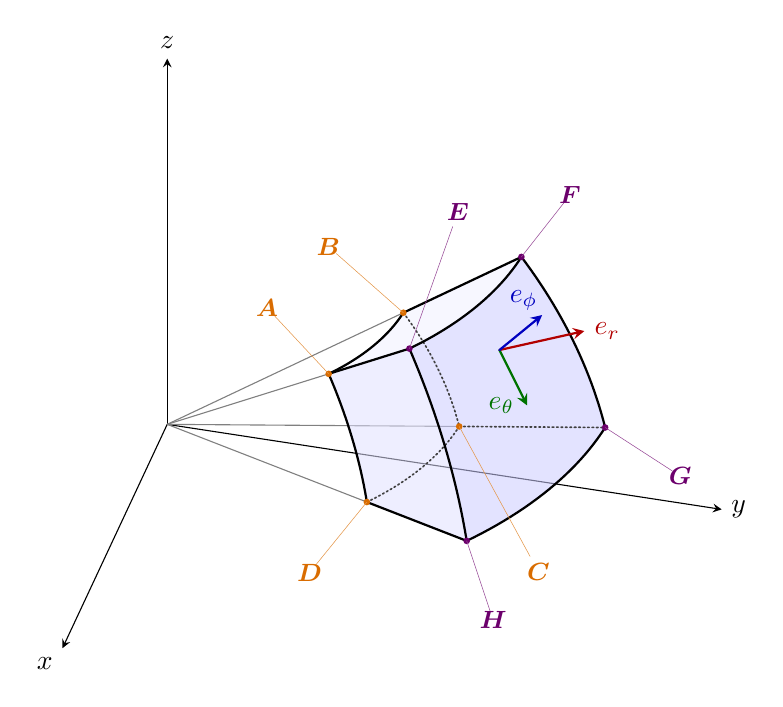
\begin{tikzpicture}[
          % orthographic view (azimuth 15 deg, elevation 35 deg), scaled by 1.35
          x={(-0.35cm,-0.748cm)}, y={(1.304cm,-0.2cm)}, z={(0cm,1.106cm)},
          line cap=round, line join=round, >=stealth,
          declare function={
            ra=3.0;  rb=4.5;     % r,     r + dr
            tha=52;  thb=77;     % theta, theta + dtheta   (polar angle, from +z)
            pa=55;   pb=85;      % phi,   phi + dphi       (azimuth, from +x)
            rm=4.5;  thm=58; pm=70;   % where the unit vectors are drawn (on the outer face)
          }]
        % one colour per coordinate direction
        \colorlet{cr}{red!70!black}
        \colorlet{cth}{green!45!black}
        \colorlet{cph}{blue!75!black}
        % vertex colours: inner face (radius r) and outer face (radius r + dr)
        \colorlet{vin}{orange!85!black}
        \colorlet{vout}{violet!85!black}

        % point at (r, theta, phi)
        \newcommand{\sph}[3]{({#1*sin(#2)*cos(#3)},{#1*sin(#2)*sin(#3)},{#1*cos(#2)})}
        % arc in theta at fixed r=#2, phi=#3, from theta=#4 to #5
        \newcommand{\tharc}[5][]{\draw[#1] plot[domain=#4:#5, samples=25, variable=\t]
            ({#2*sin(\t)*cos(#3)},{#2*sin(\t)*sin(#3)},{#2*cos(\t)});}
        % arc in phi at fixed r=#2, theta=#3, from phi=#4 to #5
        \newcommand{\pharc}[5][]{\draw[#1] plot[domain=#4:#5, samples=25, variable=\t]
            ({#2*sin(#3)*cos(\t)},{#2*sin(#3)*sin(\t)},{#2*cos(#3)});}

        % axes
        \draw[->] (0,0,0) -- (3.8,0,0) node[below left] {$x$};
        \draw[->] (0,0,0) -- (0,5.4,0) node[right] {$y$};
        \draw[->] (0,0,0) -- (0,0,4.2) node[above] {$z$};

        % rays from the origin to the four inner corners (shows the taper)
        \foreach \t/\p in {tha/pa, tha/pb, thb/pa, thb/pb}
          \draw[gray, thin] (0,0,0) -- \sph{ra}{\t}{\p};

        % visible faces: phi face (front), theta face (top), outer r face
        \fill[blue!12, opacity=0.55]
          plot[domain=tha:thb, samples=25, variable=\t] ({ra*sin(\t)*cos(pa)},{ra*sin(\t)*sin(pa)},{ra*cos(\t)})
          -- plot[domain=thb:tha, samples=25, variable=\t] ({rb*sin(\t)*cos(pa)},{rb*sin(\t)*sin(pa)},{rb*cos(\t)})
          -- cycle;
        \fill[blue!6, opacity=0.55]
          plot[domain=pa:pb, samples=25, variable=\t] ({ra*sin(tha)*cos(\t)},{ra*sin(tha)*sin(\t)},{ra*cos(tha)})
          -- plot[domain=pb:pa, samples=25, variable=\t] ({rb*sin(tha)*cos(\t)},{rb*sin(tha)*sin(\t)},{rb*cos(tha)})
          -- cycle;
        \fill[blue!20, opacity=0.55]
          plot[domain=pa:pb, samples=25, variable=\t] ({rb*sin(tha)*cos(\t)},{rb*sin(tha)*sin(\t)},{rb*cos(tha)})
          -- plot[domain=tha:thb, samples=25, variable=\t] ({rb*sin(\t)*cos(pb)},{rb*sin(\t)*sin(pb)},{rb*cos(\t)})
          -- plot[domain=pb:pa, samples=25, variable=\t] ({rb*sin(thb)*cos(\t)},{rb*sin(thb)*sin(\t)},{rb*cos(thb)})
          -- plot[domain=thb:tha, samples=25, variable=\t] ({rb*sin(\t)*cos(pa)},{rb*sin(\t)*sin(pa)},{rb*cos(\t)})
          -- cycle;

        % hidden edges (all three meet at the hidden corner C)
        \begin{scope}[densely dotted, semithick, black!75]
          \pharc{ra}{thb}{pa}{pb}
          \tharc{ra}{pb}{tha}{thb}
          \draw \sph{ra}{thb}{pb} -- \sph{rb}{thb}{pb};
        \end{scope}

        % visible edges
        \begin{scope}[thick]
          \pharc{ra}{tha}{pa}{pb}
          \pharc{rb}{tha}{pa}{pb}
          \pharc{rb}{thb}{pa}{pb}
          \tharc{ra}{pa}{tha}{thb}
          \tharc{rb}{pa}{tha}{thb}
          \tharc{rb}{pb}{tha}{thb}
          \draw \sph{ra}{tha}{pa} -- \sph{rb}{tha}{pa};
          \draw \sph{ra}{tha}{pb} -- \sph{rb}{tha}{pb};
          \draw \sph{ra}{thb}{pa} -- \sph{rb}{thb}{pa};
        \end{scope}

        % vertex labels with leader lines
        %   inner face (radius r):       A (theta, phi)   B (theta, phi+dphi)   C (theta+dtheta, phi+dphi)   D (theta+dtheta, phi)
        %   outer face (radius r + dr):  E, F, G, H directly outward from A, B, C, D
        % \dx,\dy = label offset from the vertex, in cm on the page
        \begin{scope}[font=\small\bfseries\boldmath, inner sep=1.5pt]
          \foreach \r/\t/\p/\name/\col/\dx/\dy in {
              ra/tha/pa/A/vin/-0.70/0.75,    ra/tha/pb/B/vin/-0.85/0.75,
              ra/thb/pb/C/vin/0.90/-1.65,    ra/thb/pa/D/vin/-0.65/-0.80,
              rb/tha/pa/E/vout/0.55/1.55,    rb/tha/pb/F/vout/0.55/0.70,
              rb/thb/pb/G/vout/0.85/-0.55,   rb/thb/pa/H/vout/0.30/-0.90}
          {
            \fill[\col] \sph{\r}{\t}{\p} circle[radius=1.2pt];
            \draw[very thin, \col!70] \sph{\r}{\t}{\p}
                  -- ++(\dx cm,\dy cm) node[pos=1.12, text=\col] {$\name$};
          }
        \end{scope}

        % local unit vectors
        \path \sph{rm}{thm}{pm} coordinate (M);
        \begin{scope}[shift={(M)}, thick, ->]
          \draw[cr] (0,0,0) -- ({1.15*sin(thm)*cos(pm)},{1.15*sin(thm)*sin(pm)},{1.15*cos(thm)})
                node[right] {$\pmb{e}_{r}$};
          \draw[cth] (0,0,0) -- ({0.6*cos(thm)*cos(pm)},{0.6*cos(thm)*sin(pm)},{-0.6*sin(thm)})
                node[left=1pt] {$\pmb{e}_{\theta}$};
          \draw[cph] (0,0,0) -- ({-0.7*sin(pm)},{0.7*cos(pm)},0)
                node[above left=-2pt] {$\pmb{e}_{\phi}$};
        \end{scope}
      \end{tikzpicture}%
    }
  \end{minipage}
  \caption{Infinitesimal volume element in spherical coordinates: edge lengths (left) and vertex labels (right).}
\end{figure}

Once more, apply the midpoint rule as the textbook does, meaning we measure distances relative to the midpoint of the infinitesimal wedge. We begin with the faces along the \( r \)-axis, \( ABCD \) and \( EFGH \). Their areas differ by virtue of being located at different radii along the \( \pmb{e}_{r} \) unit vector: \( r - \Delta r / 2 \) and \( r + \Delta r / 2 \). The normals for each face are
\begin{align*}
	\!\left[ \pmb{n} \, dA \right]_{ABCD} & = -\pmb{e}_{r}\!\left( r - \frac{\Delta r}{2} \right)^{2}\sin\!\left(\theta\right)\Delta \theta \Delta \phi \\
					      & = \boxed{-\pmb{e}_{r} \!\left( r^{2} - r \Delta r \right)\sin\!\left(\theta\right) \Delta \theta \Delta \phi} \\
	\!\left[ \pmb{n} \, dA \right]_{EFGH} & = \pmb{e}_{r}\!\left( r + \frac{\Delta r}{2} \right)^{2}\sin\!\left(\theta\right)\Delta \theta \Delta \phi \\
					      & = \boxed{\pmb{e}_{r}\!\left( r^{2} + r \Delta r \right)\sin\!\left(\theta\right)\Delta \theta \Delta \phi}
\end{align*}
where higher-order terms are dropped. Now we repeat the task along the other two axes, for which our work is a tad more complicated. Begin with the \( \theta \) faces \( ABFE \) and \( CDHG \). Recall first the Cartesian coordinate definitions of \( \pmb{e}_{r} \) and \( \pmb{e}_{\theta} \):
\begin{align*}
	\pmb{e}_{r}\!\left( \theta,\phi \right) & = \sin\!\left(\theta\right)\cos\!\left(\phi\right)\pmb{\hat{x}} + \sin\!\left(\theta\right)\sin\!\left(\phi\right)\pmb{\hat{y}} + \cos\!\left(\theta\right)\pmb{\hat{z}} \\
	\pmb{e}_{\theta}\!\left( \theta,\phi \right) & = \cos\!\left(\theta\right)\cos\!\left(\phi\right)\pmb{\hat{x}} + \cos\!\left(\theta\right)\sin\!\left(\phi\right)\pmb{\hat{y}} - \sin\!\left(\theta\right)\pmb{\hat{z}}
\end{align*}
where \( \partial \pmb{e}_{\theta} / \partial \theta = -\pmb{e}_{r} \). Referring to Figure 1 for the position of these faces, we see that \( ABFE \) is at \( \theta - \Delta \theta / 2 \) and \( CDHG \) at \( \theta + \Delta \theta / 2 \). We may Taylor expand \( \pmb{e}_{\theta}\!\left( \theta \pm \Delta \theta / 2,\phi \right) \) to approximate
\[
	\pmb{e}_{\theta}\!\left( \theta \pm \frac{\Delta \theta}{2},\phi \right) = \pmb{e}_{\theta}\!\left( \theta,\phi \right) \pm \frac{\Delta \theta}{2}\frac{\partial \pmb{e}_{\theta}}{\partial \theta} + \cdots = \pmb{e}_{\theta}\!\left( \theta,\phi \right) \mp \frac{\Delta \theta}{2}\pmb{e}_{r} + \cdots
\]
Ignoring the higher-order terms, look to the schematic below. The normal to face \( ABFE \) (seen here from the side along \( AE \)) is \( -\!\left[ \pmb{e}_{\theta} + \pmb{e}_{r}\!\left( \Delta \theta / 2 \right) \right] \), and to \( CDHG \), seen from the side along segment \( DH \), is \( \pmb{e}_{\theta} - \pmb{e}_{r}\!\left( \Delta \theta / 2 \right) \). The respective norms are 
\begin{align*}
	\!\left[ \pmb{n} \, dA \right]_{ABFE} & = -\!\left( \pmb{e}_{\theta} + \pmb{e}_{r}\frac{\Delta \theta}{2} \right)r \sin\!\left(\theta - \Delta \theta / 2\right) \Delta r \Delta \phi \\
				   & = -\!\left( \pmb{e}_{\theta} + \pmb{e}_{r}\frac{\Delta \theta}{2} \right)r \!\left[ \sin\!\left(\theta\right) - \frac{\Delta \theta}{2}\cos\!\left(\theta\right) \right] \Delta r \Delta \phi \\
				   & = \boxed{\pmb{e}_{\theta}\!\left[ -r \sin\!\left(\theta\right) + \frac{r \Delta \theta}{2}\cos\!\left(\theta\right) \right]\Delta r \Delta \phi - \pmb{e}_{r}\frac{r \Delta \theta}{2}\sin\!\left(\theta\right)\Delta r \Delta \phi} \\
	\!\left[ \pmb{n} \, dA \right]_{CDHG} & = \!\left( \pmb{e}_{\theta} - \pmb{e}_{r}\frac{\Delta \theta}{2} \right)r \sin\!\left(\theta + \Delta \theta / 2\right)\Delta r \Delta \phi \\
					      & = \!\left( \pmb{e}_{\theta} - \pmb{e}_{r}\frac{\Delta \theta}{2} \right)r \!\left[ \sin\!\left(\theta\right) + \frac{\Delta \theta}{2}\cos\!\left(\theta\right) \right]\Delta r \Delta \phi \\
					      & = \boxed{\pmb{e}_{\theta}\!\left[ r \sin\!\left(\theta\right) + \frac{r \Delta \theta}{2}\cos\!\left(\theta\right) \right]\Delta r \Delta \phi - \pmb{e}_{r}\frac{r \Delta \theta}{2}\sin\!\left(\theta\right)\Delta r \Delta \phi}
\end{align*}

\begin{center}
\begin{adjustbox}{max width=\linewidth}
\begin{tikzpicture}[
    >=stealth, line cap=round, line join=round,
    declare function={
      ra=3.6; rb=5.6; rm=4.6;   % r - dr/2, r + dr/2, center radius
      tha=30; thb=70; thm=50;   % theta - dtheta/2, theta + dtheta/2, center (polar angle from +z)
      hd=20;                    % half-angle dtheta/2 (exaggerated for visibility)
      L=1.4;                    % drawn length of the unit normals
    }]
  \def\D{\Delta}   % change to d for differentials
  % same colour scheme as the 3D figures
  \colorlet{cr}{red!70!black}
  \colorlet{cth}{green!45!black}
  \colorlet{cph}{blue!75!black}
  \colorlet{vin}{orange!85!black}
  \colorlet{vout}{violet!85!black}

  % Meridional half-plane phi = const: horizontal axis is the distance from the
  % z-axis, vertical axis is z.  The point (r,theta) sits at TikZ polar (90-theta : r);
  % e_r points along angle 90-theta, e_theta along angle -theta.

  % axes and the rays theta = const through the two theta-faces
  \draw[->] (0,0) -- (6.6,0) node[right] {$\rho = r\sin\theta$};
  \draw[->] (0,0) -- (0,6.2) node[above] {$z$};
  \draw[gray, dashed] (0,0) -- ({90-tha}:{rb+0.5});
  \draw[gray, dashed] (0,0) -- ({90-thb}:{rb+0.5});
  \draw[gray, densely dotted] (0,0) -- ({90-thm}:{rm});

  % angle markers (theta is measured from the z-axis)
  \draw[->] (90:0.9) arc[start angle=90, end angle={90-thm}, radius=0.9];
  \node at ({90-thm/2}:1.2) {$\theta$};
  \draw[<->, cth, thick] ({90-tha}:1.9) arc[start angle={90-tha}, end angle={90-thb}, radius=1.9];
  \node[text=cth] at ({90-thm-14}:2.45) {$\D\theta$};

  % distance of each theta-face from the z-axis (sets the face's width in phi)
  \draw[gray, thin, densely dashed] (0,{rm*cos(tha)}) -- ({90-tha}:{rm});
  \draw[gray, thin, densely dashed] (0,{rm*cos(thb)}) -- ({90-thb}:{rm});
  \node[left, font=\small] at (0,{rm*cos(tha)}) {$r\sin\bigl(\theta-\tfrac{\D\theta}{2}\bigr)$};
  \node[left, font=\small] at (0,{rm*cos(thb)}) {$r\sin\bigl(\theta+\tfrac{\D\theta}{2}\bigr)$};

  % the element in cross-section (front phi-face ADHE)
  \filldraw[thick, fill=blue!12]
    ({90-tha}:{ra}) arc[start angle={90-tha}, end angle={90-thb}, radius=ra]
    -- ({90-thb}:{rb}) arc[start angle={90-thb}, end angle={90-tha}, radius=rb] -- cycle;

  % vertices (B, C, G, F lie directly behind A, D, H, E)
  \begin{scope}[font=\small\bfseries\boldmath]
    \fill[vin]  ({90-tha}:{ra}) circle[radius=1.2pt] node[above left=-1pt, text=vin]  {$A$};
    \fill[vin]  ({90-thb}:{ra}) circle[radius=1.2pt] node[below left=-1pt, text=vin]  {$D$};
    \fill[vout] ({90-tha}:{rb}) circle[radius=1.2pt] node[above right=-1pt, text=vout] {$E$};
    \fill[vout] ({90-thb}:{rb}) circle[radius=1.2pt] node[below right=-1pt, text=vout] {$H$};
  \end{scope}

  % basis vectors at the center of the element (e_phi points into the page)
  \coordinate (O) at ({90-thm}:{rm});
  \fill (O) circle[radius=1.2pt];
  \draw[->, thick, cr]  (O) -- ++({90-thm}:0.6) node[above left=-3pt, font=\small] {$\pmb{e}_r$};
  \draw[->, thick, cth] (O) -- ++({-thm}:0.6)   node[below=-1pt, font=\small] {$\pmb{e}_\theta$};
  \begin{scope}[shift={($(O)+({180-thm/2}:0.55)$)}, cph]
    \draw[thick] (0,0) circle[radius=0.13];
    \draw[thick] (-0.092,-0.092) -- (0.092,0.092) (-0.092,0.092) -- (0.092,-0.092);
    \node[left=2pt, font=\small] at (0,0) {$\pmb{e}_\phi$};
  \end{scope}

  % --- normal on the face theta - dtheta/2 (ABFE, seen edge-on as AE): n = -e_theta there ---
  \coordinate (P) at ({90-tha}:{rm});
  \draw[->, cth, dashed] (P) -- ++({180-thm}:{L*cos(hd)}) coordinate (P1)
        node[midway, above right=-3pt, font=\small] {$-\pmb{e}_\theta$};
  \draw[->, cr, thick] (P1) -- ++({270-thm}:{L*sin(hd)})
        node[pos=0.3, above left=-2pt, font=\small] {$-\tfrac{\D\theta}{2}\pmb{e}_r$};
  \draw[->, very thick] (P) -- ++({180-tha}:{L})
        node[pos=0.7, below left=-2pt, font=\small] {$\pmb{n}_{ABFE}$};

  % --- normal on the face theta + dtheta/2 (DCGH, seen edge-on as DH): n = +e_theta there ---
  \coordinate (Q) at ({90-thb}:{rm});
  \draw[->, cth, dashed] (Q) -- ++({-thm}:{L*cos(hd)}) coordinate (Q1)
        node[midway, above right=-3pt, font=\small] {$\pmb{e}_\theta$};
  \draw[->, cr, thick] (Q1) -- ++({270-thm}:{L*sin(hd)})
        node[midway, right=1pt, font=\small] {$-\tfrac{\D\theta}{2}\pmb{e}_r$};
  \draw[->, very thick] (Q) -- ++({-thb}:{L})
        node[pos=0.8, left=1pt, font=\small] {$\pmb{n}_{DCGH}$};

  % --- inset: the two normals added tip to tail (tucked into the free upper-right corner) ---
  \begin{scope}[shift={(8.7,4.1)}]
    \node[font=\small, align=center] at (-1.0,1.95) {sum of the two\\ $\theta$-face normals};
    \coordinate (S) at (0,0);
    \draw[->, very thick] (S) -- ++({180-tha}:{1.6*L}) coordinate (S1)
          node[midway, above right=-1pt, font=\small] {$\pmb{n}_{ABFE}$};
    \draw[->, very thick] (S1) -- ++({-thb}:{1.6*L}) coordinate (S2)
          node[midway, left=3pt, font=\small] {$\pmb{n}_{DCGH}$};
    \draw[->, cr, very thick] (S) -- (S2);
    \node[cr, font=\small, anchor=north] at (-1.0,-1.35)
          {$\pmb{n}_{ABFE}+\pmb{n}_{DCGH}\approx-\D\theta\,\pmb{e}_r$};
  \end{scope}
\end{tikzpicture}
\end{adjustbox}
\end{center}

Lastly, we compute the normals for the \( \phi \) faces. The faces \( ADHE \) and \( BCGF \) are at along the azimuthal angles \( \phi - \Delta \phi / 2 \) and \( \phi + \Delta \phi / 2 \), respectively. Analogous to our method in the \( \theta \) faces, we appeal to the Cartesian definition of \( \pmb{e}_{\phi}\!\left( \phi \right) \)
\[
	\pmb{e}_{\phi}\!\left( \phi \right) = -\sin\!\left(\phi\right)\pmb{\hat{x}} + \cos\!\left(\phi\right)\pmb{\hat{y}} 
\]
and Taylor expand \( \pmb{e}_{\phi}\!\left( \phi \pm \Delta \phi / 2 \right) \) to find
\begin{align*}
	\pmb{e}_{\phi}\!\left( \phi \pm \frac{\Delta \phi}{2} \right) & = \pmb{e}_{\phi}\!\left( \phi \right) \pm \frac{\Delta \phi}{2}\frac{\partial \pmb{e}_{\phi}}{\partial \phi} \\
								      & = \pmb{e}_{\phi}\!\left( \phi \right) \mp \frac{\Delta \phi}{2}\!\left[ \sin\!\left(\theta\right)\pmb{e}_{r} + \cos\!\left(\theta\right)\pmb{e}_{\theta} \right]
\end{align*}
which we see agrees with the geometry in the figure below. The normals along the aforementioned faces are thus
\begin{align*}
	\!\left[ \pmb{n} \, dA \right]_{ADHE} & = \boxed{-\!\left[ \pmb{e}_{\phi} + \pmb{e}_{r}\frac{\Delta \phi}{2}\sin\!\left(\theta\right) + \pmb{e}_{\theta}\frac{\Delta \phi}{2}\cos\!\left(\theta\right) \right]r \Delta r \Delta \theta} \\
	\!\left[ \pmb{n} \, dA \right]_{BCGF} & = \boxed{\!\left[ \pmb{e}_{\phi} - \pmb{e}_{r}\frac{\Delta \phi}{2}\sin\!\left(\theta\right) - \pmb{e}_{\theta}\frac{\Delta \phi}{2}\cos\!\left(\theta\right) \right]r \Delta r \Delta \theta}
\end{align*}

\begin{center}
\begin{adjustbox}{max width=\linewidth}
\begin{tikzpicture}[
    >=stealth, line cap=round, line join=round,
    declare function={
      ra=3.6; rb=5.6; rm=4.6;   % rho - drho/2, rho + drho/2, center distance from the z-axis
      pa=20;  pb=60;  pm=40;    % phi - dphi/2, phi + dphi/2, center azimuth (from +x)
      hd=20;                    % half-angle dphi/2 (exaggerated for visibility)
      L=1.4;                    % drawn length of the unit normals
    }]
  \def\D{\Delta}   % change to d for differentials
  % same color scheme as the 3D figures
  \colorlet{cr}{red!70!black}
  \colorlet{cth}{green!45!black}
  \colorlet{cph}{blue!75!black}
  \colorlet{crho}{black!70}     % the horizontal direction sin(theta) e_r + cos(theta) e_theta
  \colorlet{vin}{orange!85!black}
  \colorlet{vout}{violet!85!black}

  % View straight down the z-axis.  The phi-faces are the flat half-planes phi = const,
  % seen edge-on as the two straight radial sides.  e_phi lies in this plane along angle
  % phi + 90.  The horizontal direction away from the z-axis (angle phi) is
  % sin(theta) e_r + cos(theta) e_theta; e_r and e_theta themselves point out of / into the page.

  % axes and the rays phi = const through the two phi-faces
  \draw[->] (0,0) -- (6.8,0) node[right] {$x$};
  \draw[->] (0,0) -- (0,6.2) node[above] {$y$};
  \draw[gray, dashed] (0,0) -- ({pa}:{rb+0.5});
  \draw[gray, dashed] (0,0) -- ({pb}:{rb+0.5});
  \draw[gray, densely dotted] (0,0) -- ({pm}:{rm});

  % angle markers
  \draw[->] (0:0.9) arc[start angle=0, end angle=pm, radius=0.9];
  \node at ({pm/2}:1.2) {$\phi$};
  \draw[<->, cph, thick] ({pa}:1.9) arc[start angle=pa, end angle=pb, radius=1.9];
  \node[text=cph] at ({pm+14}:2.45) {$\D\phi$};

  % the element seen from above (top theta-face ABFE)
  \filldraw[thick, fill=blue!12]
    ({pa}:{ra}) arc[start angle=pa, end angle=pb, radius=ra]
    -- ({pb}:{rb}) arc[start angle=pb, end angle=pa, radius=rb] -- cycle;

  % vertices (D, C, G, H lie directly below A, B, F, E)
  \begin{scope}[font=\small\bfseries\boldmath]
    \fill[vin]  ({pa}:{ra}) circle[radius=1.2pt] node[below left=-1pt, text=vin]  {$A$};
    \fill[vin]  ({pb}:{ra}) circle[radius=1.2pt] node[above left=-1pt, text=vin]  {$B$};
    \fill[vout] ({pa}:{rb}) circle[radius=1.2pt] node[below right=-1pt, text=vout] {$E$};
    \fill[vout] ({pb}:{rb}) circle[radius=1.2pt] node[above right=-1pt, text=vout] {$F$};
  \end{scope}

  % basis at the center of the element (e_phi in the plane; e_r and e_theta both project
  % onto the outward horizontal direction, drawn as one arrow)
  \coordinate (O) at ({pm}:{rm});
  \fill (O) circle[radius=1.2pt];
  \draw[->, thick, cph]  (O) -- ++({pm+90}:0.6) node[above left=-3pt, font=\small] {$\pmb{e}_\phi$};
  \draw[->, thick, crho] (O) -- ++({pm}:1.55)
        node[right=-1pt, font=\small, align=left] {$\sin\theta\,\pmb{e}_r+\cos\theta\,\pmb{e}_\theta$};

  % --- normal on the face phi - dphi/2 (ADHE, seen edge-on as AE): n = -e_phi there ---
  \coordinate (P) at ({pa}:{rm});
  \draw[->, cph, dashed] (P) -- ++({pm-90}:{L*cos(hd)}) coordinate (P1)
        node[midway, above right=-3pt, font=\small] {$-\pmb{e}_\phi$};
  \draw[->, crho, thick] (P1) -- ++({pm+180}:{L*sin(hd)})
        node[midway, right=1pt, font=\small] {$-\tfrac{\D\phi}{2}\bigl(\sin\theta\,\pmb{e}_r+\cos\theta\,\pmb{e}_\theta\bigr)$};
  \draw[->, very thick] (P) -- ++({pa-90}:{L})
        node[pos=0.8, left=1pt, font=\small] {$\pmb{n}_{ADHE}$};

  % --- normal on the face phi + dphi/2 (BCGF, seen edge-on as BF): n = +e_phi there ---
  \coordinate (Q) at ({pb}:{rm});
  \draw[->, cph, dashed] (Q) -- ++({pm+90}:{L*cos(hd)}) coordinate (Q1)
        node[midway, above right=-3pt, font=\small] {$\pmb{e}_\phi$};
  \draw[->, crho, thick] (Q1) -- ++({pm+180}:{L*sin(hd)})
        node[pos=0.3, above left=-2pt, font=\small] {$-\tfrac{\D\phi}{2}\bigl(\sin\theta\,\pmb{e}_r+\cos\theta\,\pmb{e}_\theta\bigr)$};
  \draw[->, very thick] (Q) -- ++({pb+90}:{L})
        node[pos=0.7, below left=-2pt, font=\small] {$\pmb{n}_{BCGF}$};

  % --- inset: the two normals added tip to tail ---
  \begin{scope}[shift={(9.4,4.3)}]
    \node[font=\small, align=center] at (-1.0,1.95) {sum of the two\\ $\phi$-face normals};
    \coordinate (S) at (0,0);
    \draw[->, very thick] (S) -- ++({pb+90}:{1.6*L}) coordinate (S1)
          node[midway, above right=-1pt, font=\small] {$\pmb{n}_{BCGF}$};
    \draw[->, very thick] (S1) -- ++({pa-90}:{1.6*L}) coordinate (S2)
          node[midway, left=3pt, font=\small] {$\pmb{n}_{ADHE}$};
    \draw[->, crho, very thick] (S) -- (S2);
    \node[crho, font=\small, anchor=north, align=center] at (-1.0,-1.35)
          {$\pmb{n}_{BCGF}+\pmb{n}_{ADHE}$\\ $\approx-\D\phi\bigl(\sin\theta\,\pmb{e}_r+\cos\theta\,\pmb{e}_\theta\bigr)$};
  \end{scope}
\end{tikzpicture}
\end{adjustbox}
\end{center}

The final step is to find the Taylor expansions of \( \pmb{Q}\!\left( r,\theta,\phi \right) \) at each of the six faces, and compute the dot product with the normals. In general, for a variable \( \alpha \), we have
\[
	\pmb{Q}\!\left( \alpha \pm \frac{\Delta \alpha}{2} \right) = \pmb{Q}\!\left( \alpha \right) \pm \frac{\partial \pmb{Q}}{\partial \alpha}\frac{\Delta \alpha}{2}
\]
Moreover, from the component definition of \( \pmb{Q}\!\left( r,\theta,\phi \right) \)
\[
	\pmb{Q}\!\left( r,\theta,\phi \right) = \pmb{e}_{r}Q_{r} + \pmb{e}_{\theta}Q_{\theta} + \pmb{e}_{\phi}Q_{\phi}
\]
we compute derivatives
\begin{align*}
	\frac{\partial \pmb{Q}}{\partial r} & = \pmb{e}_{r}\frac{\partial Q_{r}}{\partial r} + \pmb{e}_{\theta}\frac{\partial Q_{\theta}}{\partial r} + \pmb{e}_{\phi}\frac{\partial Q_{\phi}}{\partial r} \\
	\frac{\partial \pmb{Q}}{\partial \theta} & = \!\left( \pmb{e}_{r}\frac{\partial Q_{r}}{\partial \theta} + \frac{\partial \pmb{e}_{r}}{\partial \theta}Q_{r} \right) + \!\left( \pmb{e}_{\theta}\frac{\partial Q_{\theta}}{\partial \theta} + \frac{\partial \pmb{e}_{\theta}}{\partial \theta}Q_{\theta} \right) + \pmb{e}_{\phi}\frac{\partial Q_{\phi}}{\partial \theta} \\
						 & = \pmb{e}_{r}\!\left( \frac{\partial Q_{r}}{\partial \theta} - Q_{\theta} \right) + \pmb{e}_{\theta}\!\left( \frac{\partial Q_{\theta}}{\partial \theta} + Q_{r} \right) + \pmb{e}_{\phi}\frac{\partial Q_{\phi}}{\partial \theta} \\
	\frac{\partial \pmb{Q}}{\partial \phi} & = \!\left( \pmb{e}_{r}\frac{\partial Q_{r}}{\partial \phi} + \frac{\partial \pmb{e}_{r}}{\partial \phi}Q_{r} \right) + \!\left( \pmb{e}_{\theta}\frac{\partial Q_{\theta}}{\partial \phi} + \frac{\partial \pmb{e}_{\theta}}{\partial \phi}Q_{\theta} \right) + \!\left( \pmb{e}_{\phi}\frac{\partial Q_{\phi}}{\partial \phi} + \frac{\partial \pmb{e}_{\phi}}{\partial \phi}Q_{\phi} \right) \\
					       & = \pmb{e}_{r}\!\left( \frac{\partial Q_{r}}{\partial \phi} - Q_{\phi}\sin\!\left(\theta\right) \right) + \pmb{e}_{\theta}\!\left( \frac{\partial Q_{\theta}}{\partial \phi} - Q_{\phi}\cos\!\left(\theta\right) \right) \\
					       & \qquad + \pmb{e}_{\phi}\!\left( \frac{\partial Q_{\phi}}{\partial \phi} + Q_{r}\sin\!\left(\theta\right) + Q_{\theta}\cos\!\left(\theta\right) \right)
\end{align*}

We finally have what we need for the penultimate step of computing dot products:
\begin{align*}
	\!\left[ \pmb{n} \cdot \pmb{Q} \, dA \right]_{ABCD} & = \!\left[ \pmb{Q} - \frac{\partial \pmb{Q}}{\partial r}\frac{\Delta r}{2} \right] \cdot \!\left[ -\pmb{e}_{r}\!\left( r^{2} - r \Delta r \right)\sin\!\left(\theta\right)\Delta \theta \Delta \phi \right] \\
	 & = -Q_{r}\!\left( r^{2} - r \Delta r \right)\sin\!\left(\theta\right)\Delta \theta \Delta \phi \\
	 & \qquad + \frac{\partial Q_{r}}{\partial r}\frac{\Delta r}{2}\!\left( r^{2} - r \Delta r \right)\sin\!\left(\theta\right)\Delta \theta \Delta \phi \\ 
	 & = -Q_{r}\!\left( r^{2} - r \Delta r \right)\sin\!\left(\theta\right)\Delta \theta \Delta \phi \\
	 & \qquad + \frac{1}{2}\frac{\partial Q_{r}}{\partial r}r^{2}\sin\!\left(\theta\right)\Delta r \Delta \theta \Delta \phi \\
	\!\left[ \pmb{n} \cdot \pmb{Q} \, dA \right]_{EFGH} & = \!\left( \pmb{Q} + \frac{\partial \pmb{Q}}{\partial r}\frac{\Delta r}{2} \right) \cdot \pmb{e}_{r}\!\left( r^{2} + r \Delta r \right)\sin\!\left(\theta\right)\Delta \theta \Delta \phi \\
	 & = Q_{r}\!\left( r^{2} + r \Delta r \right)\sin\!\left(\theta\right)\Delta \theta \Delta \phi \\
	 & \qquad + \frac{\partial Q_{r}}{\partial r}\frac{\Delta r}{2}\!\left( r^{2} + r \Delta r \right)\sin\!\left(\theta\right)\Delta \theta \Delta \phi \\ 
	 & = Q_{r}\!\left( r^{2} + r \Delta r \right)\sin\!\left(\theta\right)\Delta \theta \Delta \phi \\
	 & \qquad + \frac{1}{2}\frac{\partial Q_{r}}{\partial r}r^{2}\sin\!\left(\theta\right)\Delta r \Delta \theta \Delta \phi \\
	\!\left[ \pmb{n} \cdot \pmb{Q} \, dA \right]_{ABCD} & + \!\left[ \pmb{n} \cdot \pmb{Q} \, dA \right]_{EFGH} = \boxed{\!\left( \frac{2Q_{r}}{r} + \frac{\partial Q_{r}}{\partial r} \right)r^{2}\sin\!\left(\theta\right)\Delta r \Delta \theta \Delta \phi} \\
	\!\left[ \pmb{n} \cdot \pmb{Q} \, dA \right]_{ABFE} & = \!\left[ \pmb{Q} - \frac{\partial \pmb{Q}}{\partial \theta}\frac{\Delta \theta}{2} \right] \cdot \!\left[ \pmb{e}_{\theta}\!\left[ -r \sin\!\left(\theta\right) + \frac{r \Delta \theta}{2}\cos\!\left(\theta\right) \right]\Delta r \Delta \phi - \pmb{e}_{r}\frac{r \Delta \theta}{2}\sin\!\left(\theta\right)\Delta r \Delta \phi \right] \\
							    & = Q_{\theta}\!\left[ -r \sin\!\left(\theta\right) + \frac{r \Delta \theta}{2}\cos\!\left(\theta\right) \right]\Delta r \Delta \phi - Q_{r}\frac{r \Delta \theta}{2}\sin\!\left(\theta\right)\Delta r \Delta \phi \\
							    & \quad + \!\left( \frac{\partial Q_{\theta}}{\partial \theta} + Q_{r} \right)\frac{\Delta \theta}{2}\!\left[ r \sin\!\left(\theta\right) - \frac{r \Delta \theta}{2}\cos\!\left(\theta\right) \right]\Delta r \Delta \phi \\
							    & \qquad + \!\left( \frac{\partial Q_{r}}{\partial \theta} - Q_{\theta} \right)\frac{r \!\left( \Delta \theta \right)^{2}}{4}\sin\!\left(\theta\right)\Delta r \Delta \phi \\
							    & = -Q_{\theta}r \sin\!\left(\theta\right)\Delta r \Delta \phi + Q_{\theta}\frac{r \Delta \theta}{2}\cos\!\left(\theta\right)\Delta r \Delta \phi + \frac{1}{2r}\frac{\partial Q_{\theta}}{\partial \theta}r^{2}\sin\!\left(\theta\right)\Delta r \Delta \theta \Delta \phi \\
	\!\left[ \pmb{n} \cdot \pmb{Q} \, dA \right]_{CDHG} & = \!\left[ \pmb{Q} + \frac{\partial \pmb{Q}}{\partial \theta}\frac{\Delta \theta}{2} \right] \cdot \!\left[ \pmb{e}_{\theta}\!\left[ r \sin\!\left(\theta\right) + \frac{r \Delta \theta}{2}\cos\!\left(\theta\right) \right]\Delta r \Delta \phi - \pmb{e}_{r}\frac{r \Delta \theta}{2}\sin\!\left(\theta\right)\Delta r \Delta \phi \right] \\
							    & = Q_{\theta}\!\left[ r \sin\!\left(\theta\right) + \frac{r \Delta \theta}{2}\cos\!\left(\theta\right) \right]\Delta r \Delta \phi - Q_{r}\frac{r \Delta \theta}{2}\sin\!\left(\theta\right)\Delta r \Delta \phi \\
							    & \quad + \!\left( \frac{\partial Q_{\theta}}{\partial \theta} + Q_{r} \right)\frac{\Delta \theta}{2}\!\left[ r \sin\!\left(\theta\right) + \frac{r \Delta \theta}{2}\cos\!\left(\theta\right) \right]\Delta r \Delta \phi \\
							    & \qquad - \!\left( \frac{\partial Q_{r}}{\partial \theta} - Q_{\theta} \right)\frac{r \!\left( \Delta \theta \right)^{2}}{4}\sin\!\left(\theta\right)\Delta r \Delta \phi \\
							    & = Q_{\theta}r \sin\!\left(\theta\right)\Delta r \Delta \phi + Q_{\theta}\frac{r \Delta \theta}{2}\cos\!\left(\theta\right)\Delta r \Delta \phi + \frac{1}{2r}\frac{\partial Q_{\theta}}{\partial \theta}r^{2}\sin\!\left(\theta\right)\Delta r \Delta \theta \Delta \phi \\
	\!\left[ \pmb{n} \cdot \pmb{Q} \, dA \right]_{ABFE} & + \!\left[ \pmb{n} \cdot \pmb{Q} \, dA \right]_{CDHG} = \boxed{\!\left( \frac{Q_{\theta}}{r}\cot\!\left(\theta\right) + \frac{1}{r}\frac{\partial Q_{\theta}}{\partial \theta} \right)r^{2}\sin\!\left(\theta\right)\Delta r \Delta \theta \Delta \phi} 
\end{align*}
\begin{align*}
	\!\left[ \pmb{n} \cdot \pmb{Q} \, dA \right]_{ADHE} & = \!\left[ \pmb{Q} - \frac{\partial \pmb{Q}}{\partial \phi}\frac{\Delta \phi}{2} \right] \cdot \!\left[ -\!\left[ \pmb{e}_{\phi} + \pmb{e}_{r}\frac{\Delta \phi}{2}\sin\!\left(\theta\right) + \pmb{e}_{\theta}\frac{\Delta \phi}{2}\cos\!\left(\theta\right) \right]r \Delta r \Delta \theta \right] \\
							    & = -\!\left( Q_{r}\frac{\Delta \phi}{2}\sin\!\left(\theta\right) + Q_{\theta}\frac{\Delta \phi}{2}\cos\!\left(\theta\right) + Q_{\phi} \right)r \Delta r \Delta \theta \\
							    & \quad + \biggl[ \!\left( \frac{\partial Q_{r}}{\partial \phi} + Q_{\phi}\sin\!\left(\theta\right) \right)\!\left( \frac{\Delta \phi}{2} \right)^{2}\sin\!\left(\theta\right) + \!\left( \frac{\partial Q_{\theta}}{\partial \phi} + Q_{\phi}\cos\!\left(\theta\right) \right)\!\left( \frac{\Delta \phi}{2} \right)^{2}\cos\!\left(\theta\right) \\
							    & \qquad + \!\left( \frac{\partial Q_{\phi}}{\partial \phi} + Q_{r}\sin\!\left(\theta\right) + Q_{\theta}\cos\!\left(\theta\right) \right)\!\left( \frac{\Delta \phi}{2} \right) \biggr]r \Delta r \Delta \theta \\
							    & = -Q_{\phi}r \Delta r \Delta \theta + \frac{1}{2}\frac{\partial Q_{\phi}}{\partial \phi}r \Delta r \Delta \theta \Delta \phi  \\
	\!\left[ \pmb{n} \cdot \pmb{Q} \, dA \right]_{BCGF} & = \!\left[ \pmb{Q} + \frac{\partial \pmb{Q}}{\partial \phi}\frac{\Delta \phi}{2} \right] \cdot \!\left[ \pmb{e}_{\phi} - \pmb{e}_{r}\frac{\Delta \phi}{2}\sin\!\left(\theta\right) - \pmb{e}_{\theta}\frac{\Delta \phi}{2}\cos\!\left(\theta\right) \right]r \Delta r \Delta \theta \\
							    & = \!\left( -Q_{r}\frac{\Delta \phi}{2}\sin\!\left(\theta\right) - Q_{\theta}\frac{\Delta \phi}{2}\cos\!\left(\theta\right) + Q_{\phi} \right)r \Delta r \Delta \theta \\
							    & \quad + \biggl[ -\!\left( \frac{\partial Q_{r}}{\partial \phi} + Q_{\phi}\sin\!\left(\theta\right) \right)\!\left( \frac{\Delta \phi}{2} \right)^{2}\sin\!\left(\theta\right) - \!\left( \frac{\partial Q_{\theta}}{\partial \phi} + Q_{\phi}\cos\!\left(\theta\right) \right)\!\left( \frac{\Delta \phi}{2} \right)^{2}\cos\!\left(\theta\right) \\
							    & \qquad + \!\left( \frac{\partial Q_{\phi}}{\partial \phi} + Q_{r}\sin\!\left(\theta\right) + Q_{\theta}\cos\!\left(\theta\right) \right)\!\left( \frac{\Delta \phi}{2} \right) \biggr]r \Delta r \Delta \theta \\
							    & = Q_{\phi}r \Delta r \Delta \theta + \frac{1}{2}\frac{\partial Q_{\phi}}{\partial \phi}r \Delta r \Delta \theta \Delta \phi  \\
	\!\left[ \pmb{n} \cdot \pmb{Q} \, dA \right]_{ADHE} & + \!\left[ \pmb{n} \cdot \pmb{Q} \, dA \right]_{BCGF} = \boxed{\frac{1}{r \sin\!\left(\theta\right)}\frac{\partial Q_{\phi}}{\partial \phi}r^{2} \Delta r\sin\!\left(\theta\right) \Delta \theta \Delta \phi}
\end{align*}

At last, summing the terms produces
\begin{align*}
	\nabla \cdot \pmb{Q} & = \lim\limits_{V \to 0}\frac{1}{V}\iint_{A} \pmb{n} \cdot \pmb{Q} \, dA \\
			     & = \lim\limits_{\substack{\Delta r \to 0 \\ \Delta \theta \to 0 \\ \Delta \phi \to 0}}\frac{1}{r^{2}\sin\!\left(\theta\right)\Delta r \Delta \theta \Delta \phi}\!\left( \frac{2Q_{r}}{r} + \frac{\partial Q_{r}}{\partial r} + \frac{1}{r}\frac{\partial Q_{\theta}}{\partial \theta} + \frac{\cot\!\left(\theta\right)}{r}Q_{\theta} + \frac{1}{r \sin\!\left(\theta\right)}\frac{\partial Q_{\phi}}{\partial \phi} \right)r^{2}\sin\!\left(\theta\right)\Delta r \Delta \theta \Delta \phi \\ 
			     & = \frac{1}{r^{2}}\frac{\partial }{\partial r}\!\left( r^{2}Q_{r} \right) + \frac{1}{r \sin\!\left( \theta \right)}\frac{\partial }{\partial \theta}\!\left( \sin\!\left(\theta\right)Q_{\theta} \right) + \frac{1}{r \sin\!\left(\theta\right)}\frac{\partial Q_{\phi}}{\partial \phi}
\end{align*}

% QUESTION 21
\qs{2.21}{Use the vector integral theorems to prove that \( \nabla \cdot \!\left( \nabla \times \pmb{u} \right) = 0 \) for any twice-differentiable vector function \( \pmb{u} \) regardless of the coordinate system.}

By  Gauss's theorem,
\[
	\iiint_{V}\nabla \cdot \!\left( \nabla \times \pmb{u} \right) \, dV = \iint_{A}\pmb{n} \cdot \!\left( \nabla \times \pmb{u} \right) \, dA  
\]
Now, intuition tells us that Stokes' theorem is next, which is correct. Some nuance, however, is required. Stokes' theorem deals with an \textit{open} surface area and the bounding curve around the surface. With a closed surface, we can take an arbitrary cut through it, fix a direction, and call that our boundary curve \( C \). This produces two \textit{open} surfaces. Because the direction of that curve is fixed, the right-hand rule traverses the curve \( C \) in opposite directions on each surface and their line integrals cancel, yielding zero under Stokes' theorem. 
\[
	\iint_{A} \pmb{n} \cdot \!\left( \nabla \times \pmb{u} \right) \, dA = \oint_{C} \pmb{u} \cdot d \pmb{l} - \oint_{C} \pmb{u} \cdot d \pmb{l} = 0 
\]
Lastly, since \( V \) can be any arbitrary volume, by continuity of the integrand as established by the twice-differentiability of \( \pmb{u} \), we establish \( \nabla \cdot \!\left( \nabla \times \pmb{u} \right) = 0 \).

\end{document}
